%\setlength{\epigraphwidth}{0.5\textwidth}
%\epigraph{There is an art in the contemplation of water. It is necessary to look at it as foaming in waves.}{--- \textup{Mencius}, \textit{\\translated by James Legge}}

The SNO+ water data taking from May 2017 to September 2018. The period from May 2017 to October 2018 is the first stage of the water phase. During this stage, several calibration runs were taken, including the $^{16}$N calibration scans and the laserball scans. During the period from October 2018 to July 2019, over 20 tonnes of LAB (without PPO) was filled into the detector and the liquid mostly occupied the neck volume, slightly below the neck bottom. With the nitrogen cover gas on the top, the data taken during this period is considered as low background data.


The open dataset 100000 to 100399, from 4 to 14 May 2017.


\section{High Level Cuts: Classifiers}

A set of classifiers have been developed since the SNO analysis and been optimized for the SNO+ data \cite{highlevel}.


\begin{itemize}

\item[$\bullet$] In time ratio (ITR) classifier

This classifier calculates the ratio of the number of hits in an optimized prompt time window ([-2.5,5.0]~ns for the water phase) to the total number of hits.


\item[$\bullet$] $\beta_{14}$ isotropy classifier

This classifier uses Legendre polynomials to return the	first ($\beta_1$) and the fourth ($\beta_4$) spherical	harmonics of an event, where:
\[
\beta_l = \frac{2}{N(N-1)}\sum_{i=1}^{N-1}\sum_{j=i+1}^N P_l(\cos\theta_{ij})
\]
and $P_l(\cos\theta_{ij})$ are Legendre polynomials.

The	combination	of these two polynomials returned by the classifier	was	
practically	chosen by the SNO collaboration	to be: $\beta_{14}=\beta_1+4\beta_4$
as	this gives	something	that	looks	kinda gaussian-like	for	Cerenkov	events.	
Essentially	any	deviation	from	zero	suggests	some	polarity	(i.e.	the	event	is	not	
isotropic).	



\item[$\bullet$] $\theta_{ij}$ isotropy classifier 

describes the angle subtended at an event vertex by PMT \#i and PMT \#j.

\[
\cos\theta_{ij}=\frac{(\vec{X}_{PMT\#i}- \vec{X}_{event})\cdot (\vec{X}_{PMT\#j}- \vec{X}_{event})}{|\vec{X}_{PMT\#i}- \vec{X}_{event}||\vec{X}_{PMT\#j}- \vec{X}_{event}|}
\]
\end{itemize}


\section{\isotope[16]{N} Calibration Scans in the Water Phase}
During the water phase, an Nitrogen-16 ($^{16}$N) calibration source was deployed for internal detector calibration scans in June and November, 2017 and external detector scans in March, 2018.

The $^{16}$N calibration runs provide an ideal test of fitter performance. From a comparison of reconstructions for data and MC, we can also extract the resolution and bias of the fitter. Here I worked out the vertex and the direction reconstruction performances for both of the RAT water fitter and the MPW. The vertex shifts as well as the uncertainties are evaluated. 

The $\gamma$-rays emitted from the $^{16}$N source interact with the water in the detector mainly via Compton scattering. Figure~\ref{hsx} shows the spatial distributions of the first $\gamma$-ray interaction positions projected on the x axis (called spatial distribution $S(x)$) obtained from MC simulation. The $^{16}$N source is considered as an electron source with a known spatial distribution\cite{boulay2004direct}. For simplicity, in the following we always discuss the $x$ component of the position vector $\vec{X}$. 

\begin{figure}[!htb]
	\centering
	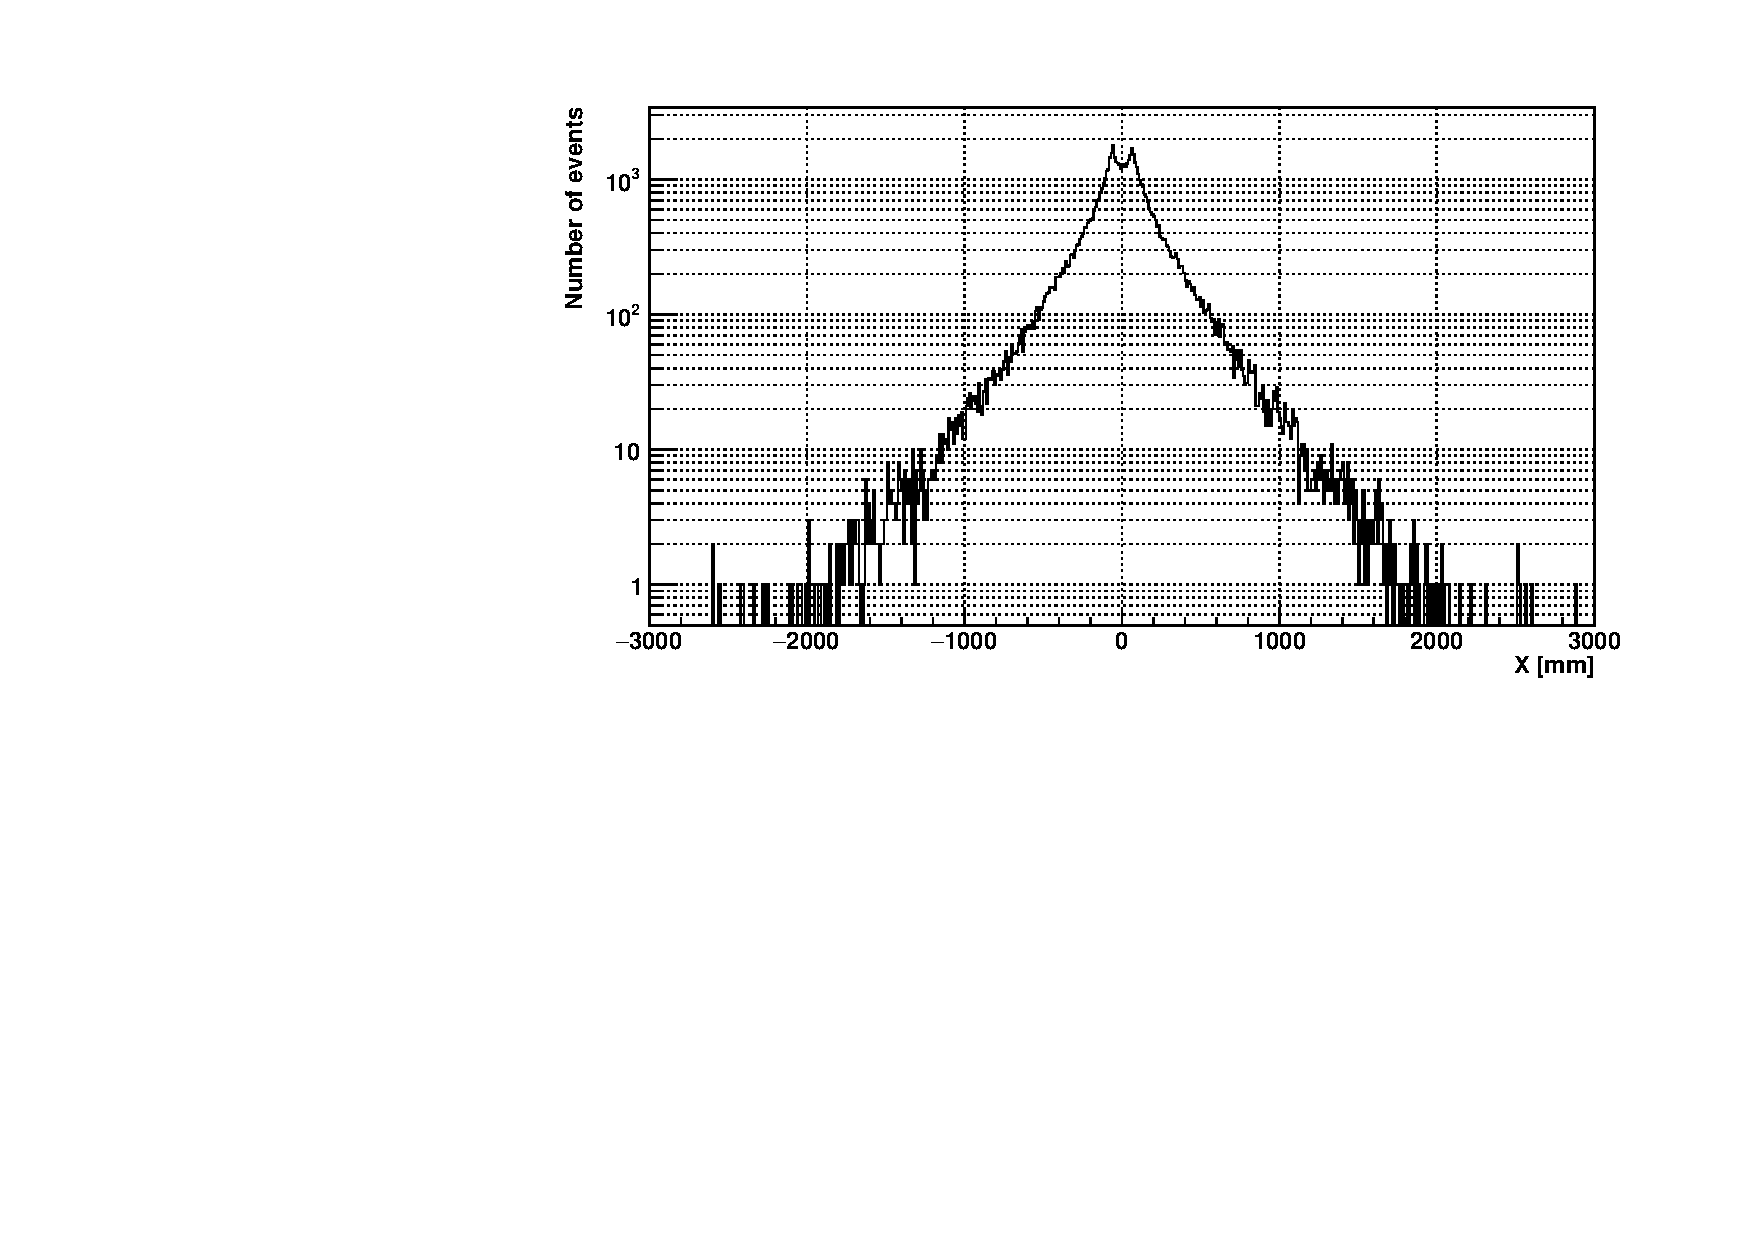
\includegraphics[width=9cm]{sx.pdf}
	\caption{Spatial distributions of {$^{16}$}N first $\gamma$-rays interaction position projected on x axis, obtained from RAT simulations. The double-peak structure is due to the wall of the stainless steel container of the $^{16}N$ source.}
	\label{hsx}
\end{figure}

A position resolution function is defined for the reconstructed electron position distribution\cite{boulay2004direct}:
\[
R(x)=\frac{1-\alpha_e}{\sqrt{2\pi}\sigma_p}\exp{[-\frac{1}{2}(\frac{x-\mu_p}{\sigma_p})^2]+\frac{\alpha_e}{2\tau_p}\exp{[\frac{-|x-\mu_p|}{\tau_p}]}},
\]
where $\alpha_e$ is the fractional exponential component, $\sigma_p$ is
the Gaussian width (corresponding to the position resolution), $\mu_p$ is the Gaussian shift  (corresponding to the position bias) and $\tau_p$ is the exponential slope (corresponding to the position distributions in tails).

For electrons from the $^{16}$N calibration source, their spatial distribution function $N_{R}(x)$ can be described by the position resolution function smeared by the convolution of $S(x)$ as\cite{boulay2004direct}:
\[
N_{R}(x)=\int^{+\infty}_{-\infty} S(x)R(x_{fit}-x)dx.
\]

Since the $S(x)$ and $N_{R}(x)$ are histograms obtained from the data and MC, we calculate by the bin value $x_i$: 
\[N_R(x_i)=\sum_{x_i=-\infty}^{+\infty}S(x_i)R(x_{fit}^i-x_i).\].

The $\chi^2$ is calculated by:
\[
\chi^2=\sum^{N_{bins}}_{i=0}[\frac{N_R(x_{fit}^i)-N_R^{fit}(x_{fit}^i)}{\sigma_i}]^2,
\]
where $N_R^{fit}$ is a trial fit to the $N_R$ by tuning the $\{\alpha_e,\mu_p,\sigma_p,\tau_p\}$ and $\sigma_i$ is taken as the bin width of the histograms.

By minimizing the $\chi^2$, the parameters of the resolution function, $\{\alpha_e,\mu_p,\sigma_p,\tau_p\}$ and a best $N_R^{fit}$ are obtained.

Fig.~\ref{posresol} shows a comparison of the reconstructed x position of {$^{16}$}N events between data and MC. The reconstructed position distributions are fitted with $N_R^{fit}$.

%\begin{figure}[!htb]
%	\centering
%	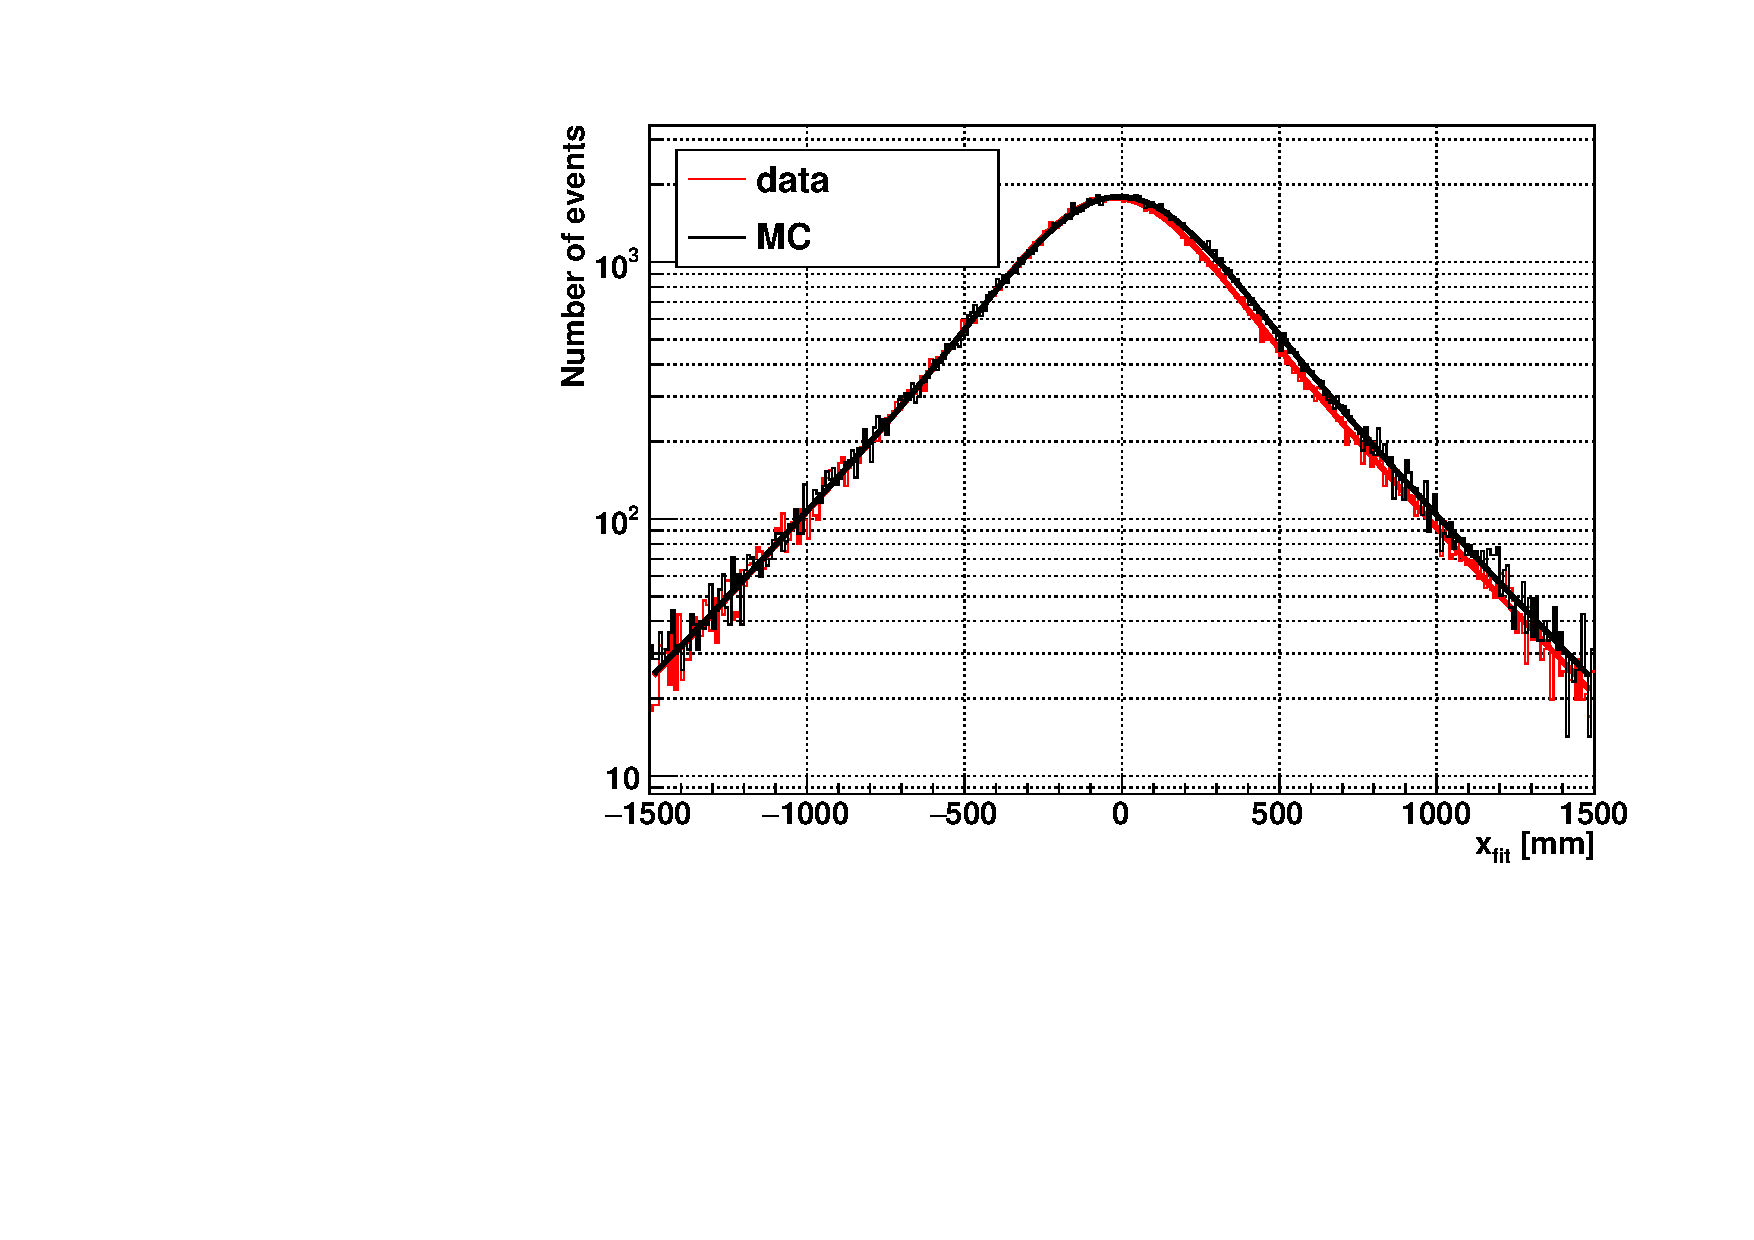
\includegraphics[width=10cm]{posResol.pdf}
%	\caption{Distributions of the reconstructed position projected on x axis, obtained from SNO+ {$^{16}$}N central run data (red) and MC (black). The distributions are fitted with $N_R^{fit}$ (red and black lines).}
%	\label{posresol}
%\end{figure}

\begin{figure}
	\centering
	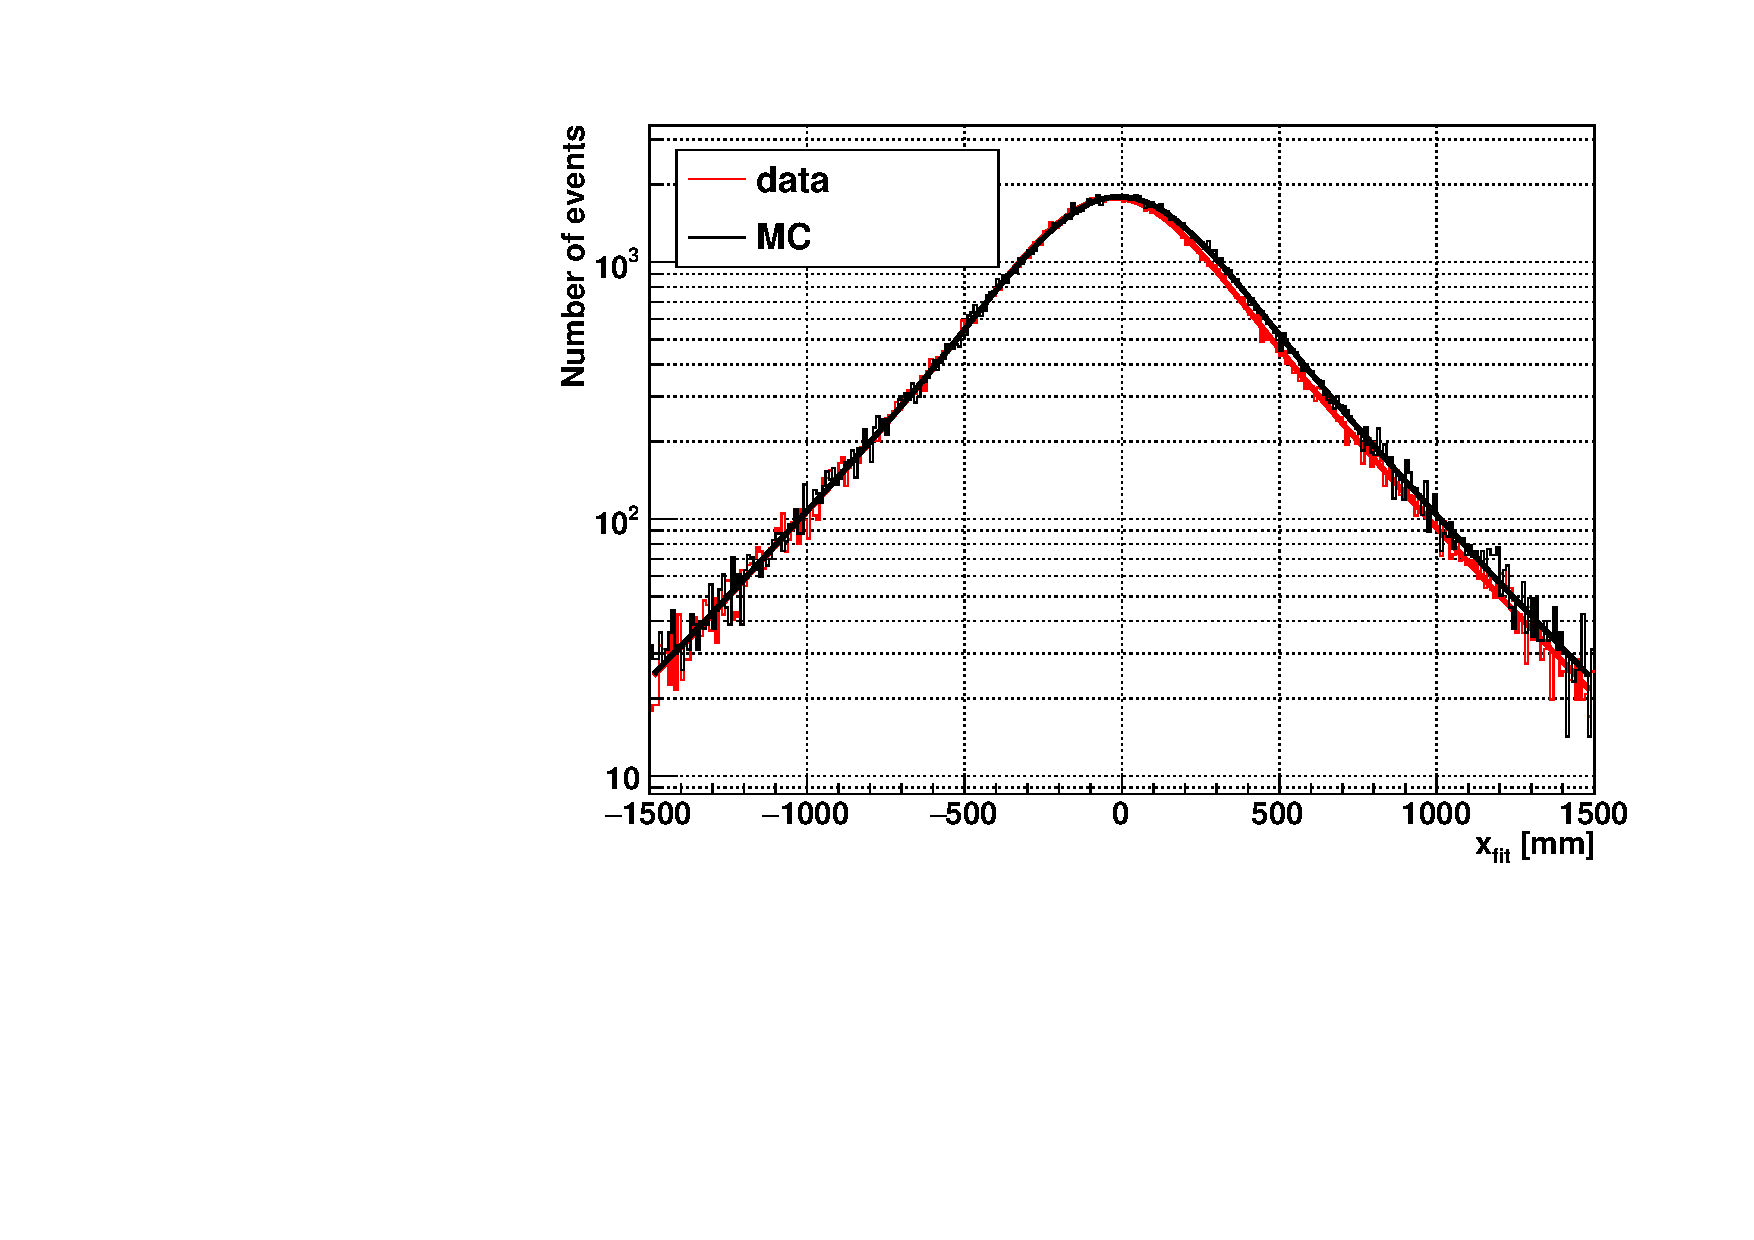
\includegraphics[width=140mm]{posResol.pdf}\label{posresol}
	\caption{Position resolutions, compared the data (red) and MC (black). The resolution fit functions are overlaid with histograms.}
\end{figure}

Table~\ref{table_posresol} summarizes the values of position resolution parameters obtained from data and MC of {$^{16}$}N calibration runs at the detector center.
\vspace{1mm}
\begin{table}[ht]
	\centering
	\caption{Position resolution parameters for the MP Water Fitter.}
	\label{table_posresol}
	\begin{tabular}{ccccc}
		\toprule
		MPW fitter & $\alpha_e$ & $\sigma_P$ (mm) &  $\tau_P$ (mm)& $\mu_P$ (mm)\\
		\hline 
		data& 0.58$\pm$0.04 & 175.8$\pm$3.8 & 288.0$\pm$5.7 & -28.8$\pm$1.0\\	
		\hline 
		MC & 0.51$\pm$0.05 & 195.2$\pm$3.3 & 298.4$\pm$6.1 & -10.9$\pm$1.0\\
		\bottomrule
	\end{tabular}
\end{table}
\vspace{1mm}

Vertex likelihood surface for an typical {$^{16}$}N event (calibration run-100934\_s000\_p001, event GTID = 61836), projected on X-Y, X-Z and Y-Z planes. A clean global maxima gives the reconstructed vertex: the fitted position is at (-211.958, 503.399, 275.990) mm and the fitted time at 217.03885 ns. This is shown in Fig.~\ref{likelihoodSurface}. 

\begin{figure}
	\centering
	%\subfigure[X-Y plane.]{\label{fig:1a}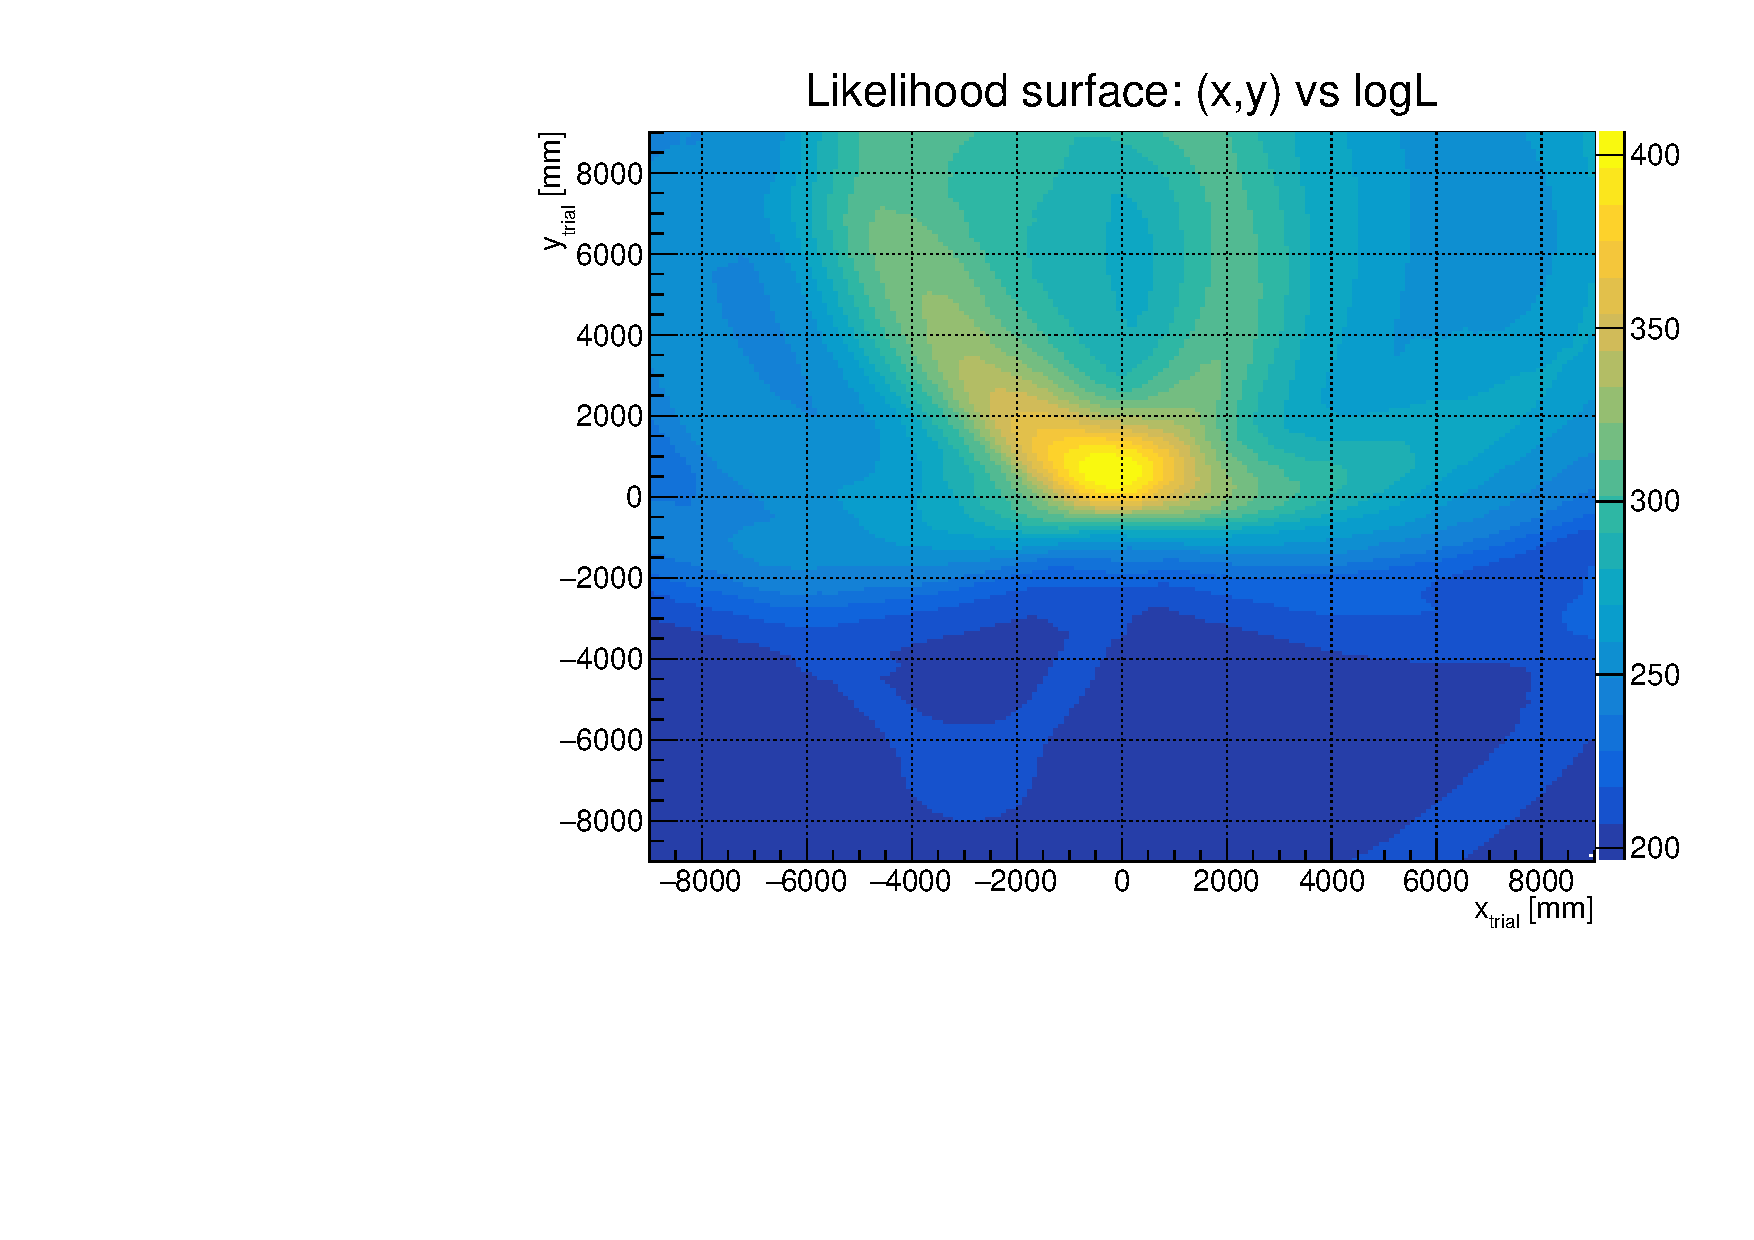
\includegraphics[width=65mm]{likelihoodSurface_xy.pdf}}
	%\subfigure[Y-Z plane.]{\label{fig:1b}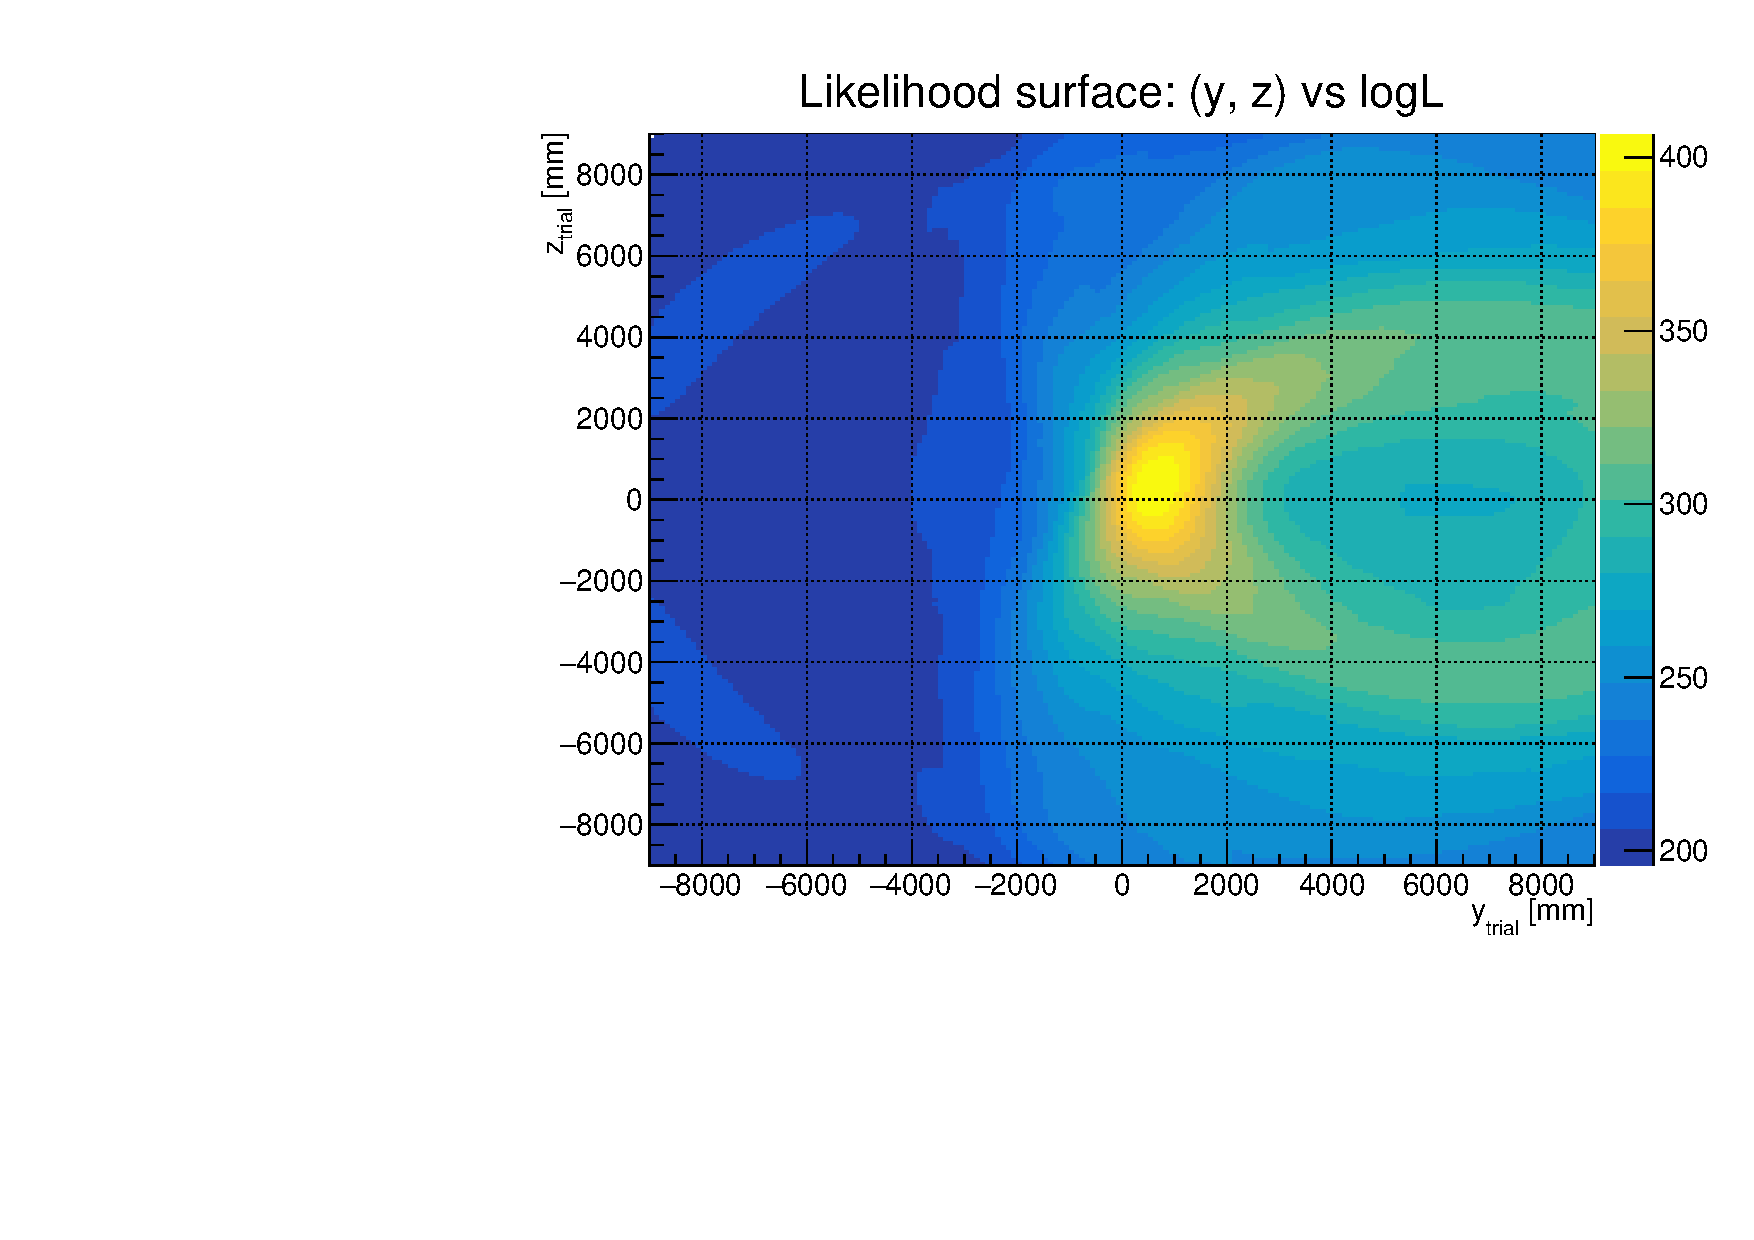
\includegraphics[width=65mm]{likelihoodSurface_yz.pdf}}
	%\subfigure[X-Z plane.]{\label{fig:1c}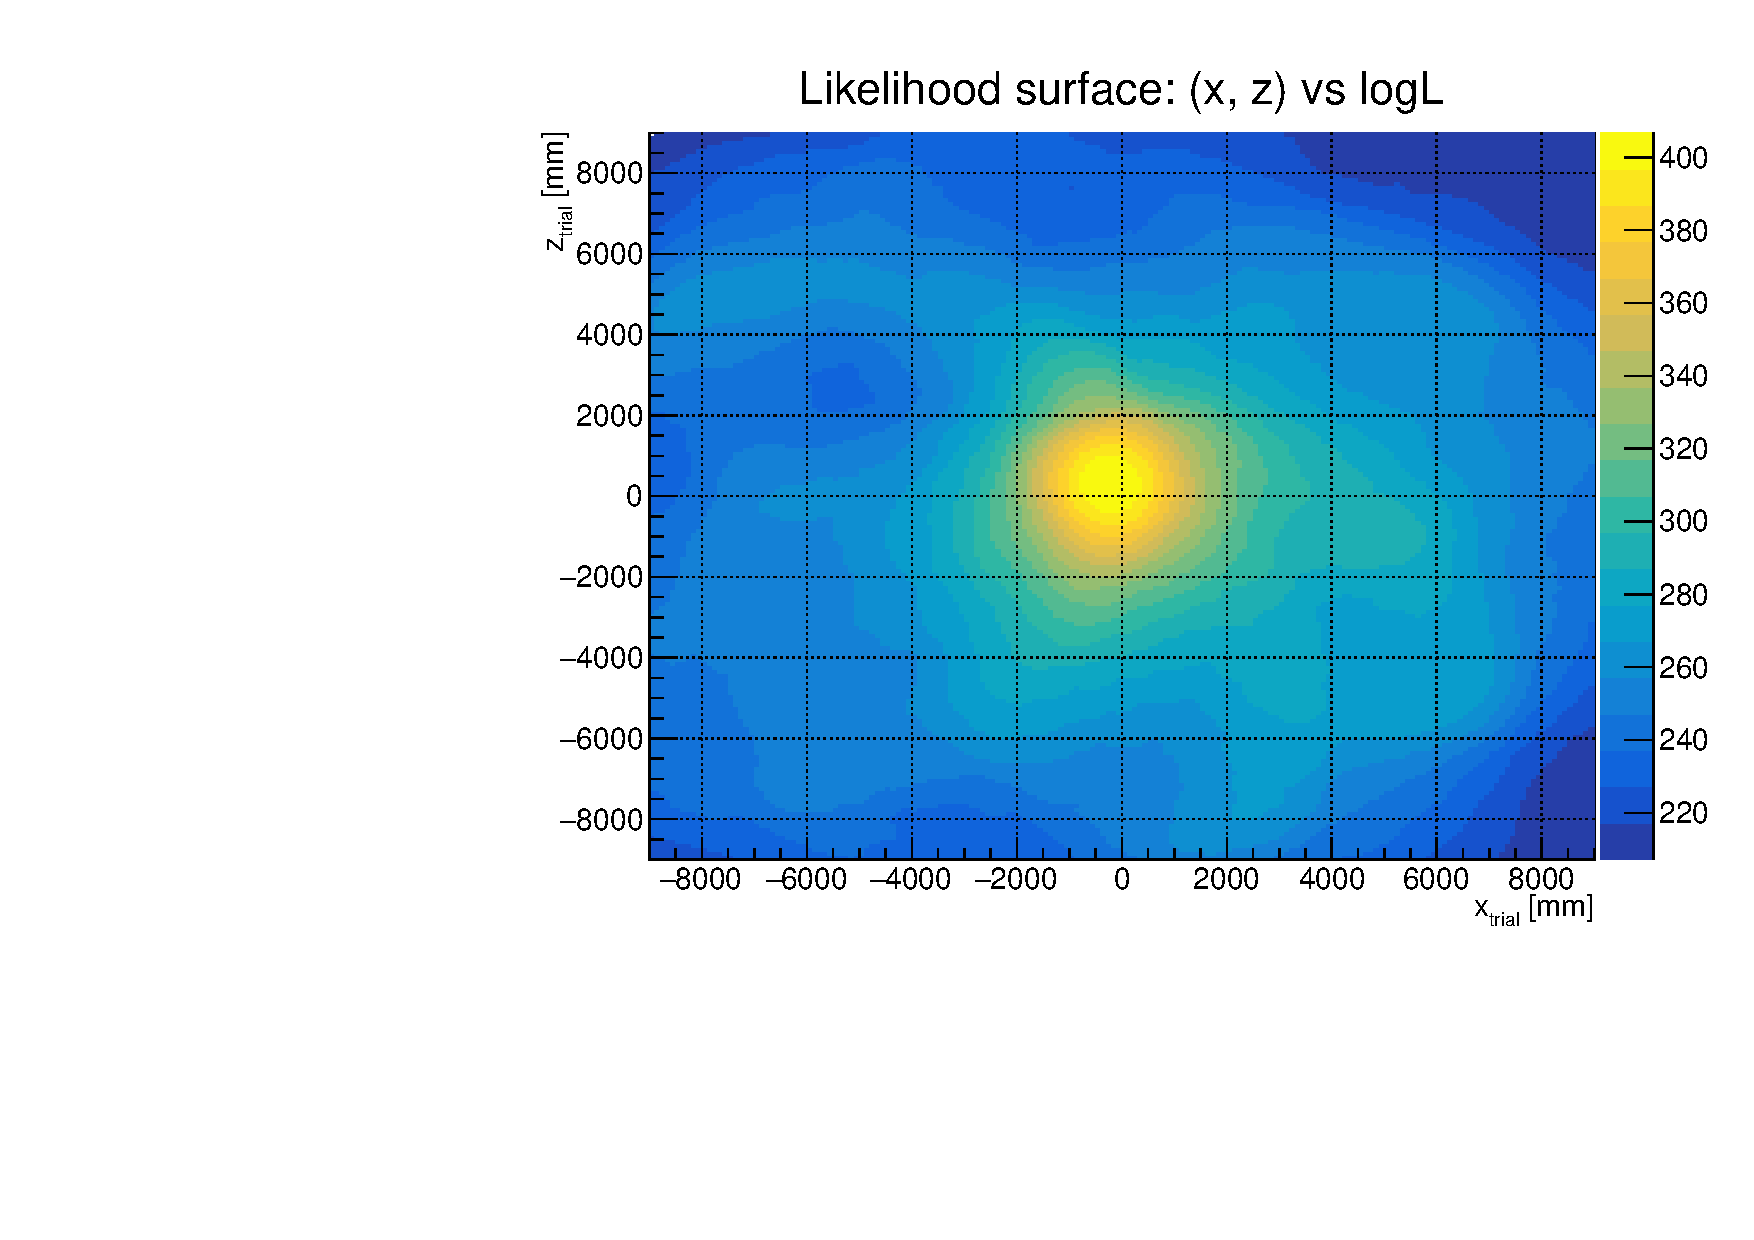
\includegraphics[width=65mm]{likelihoodSurface_xz.pdf}}
	\subfigure[X-Y plane.]{\label{fig:1a}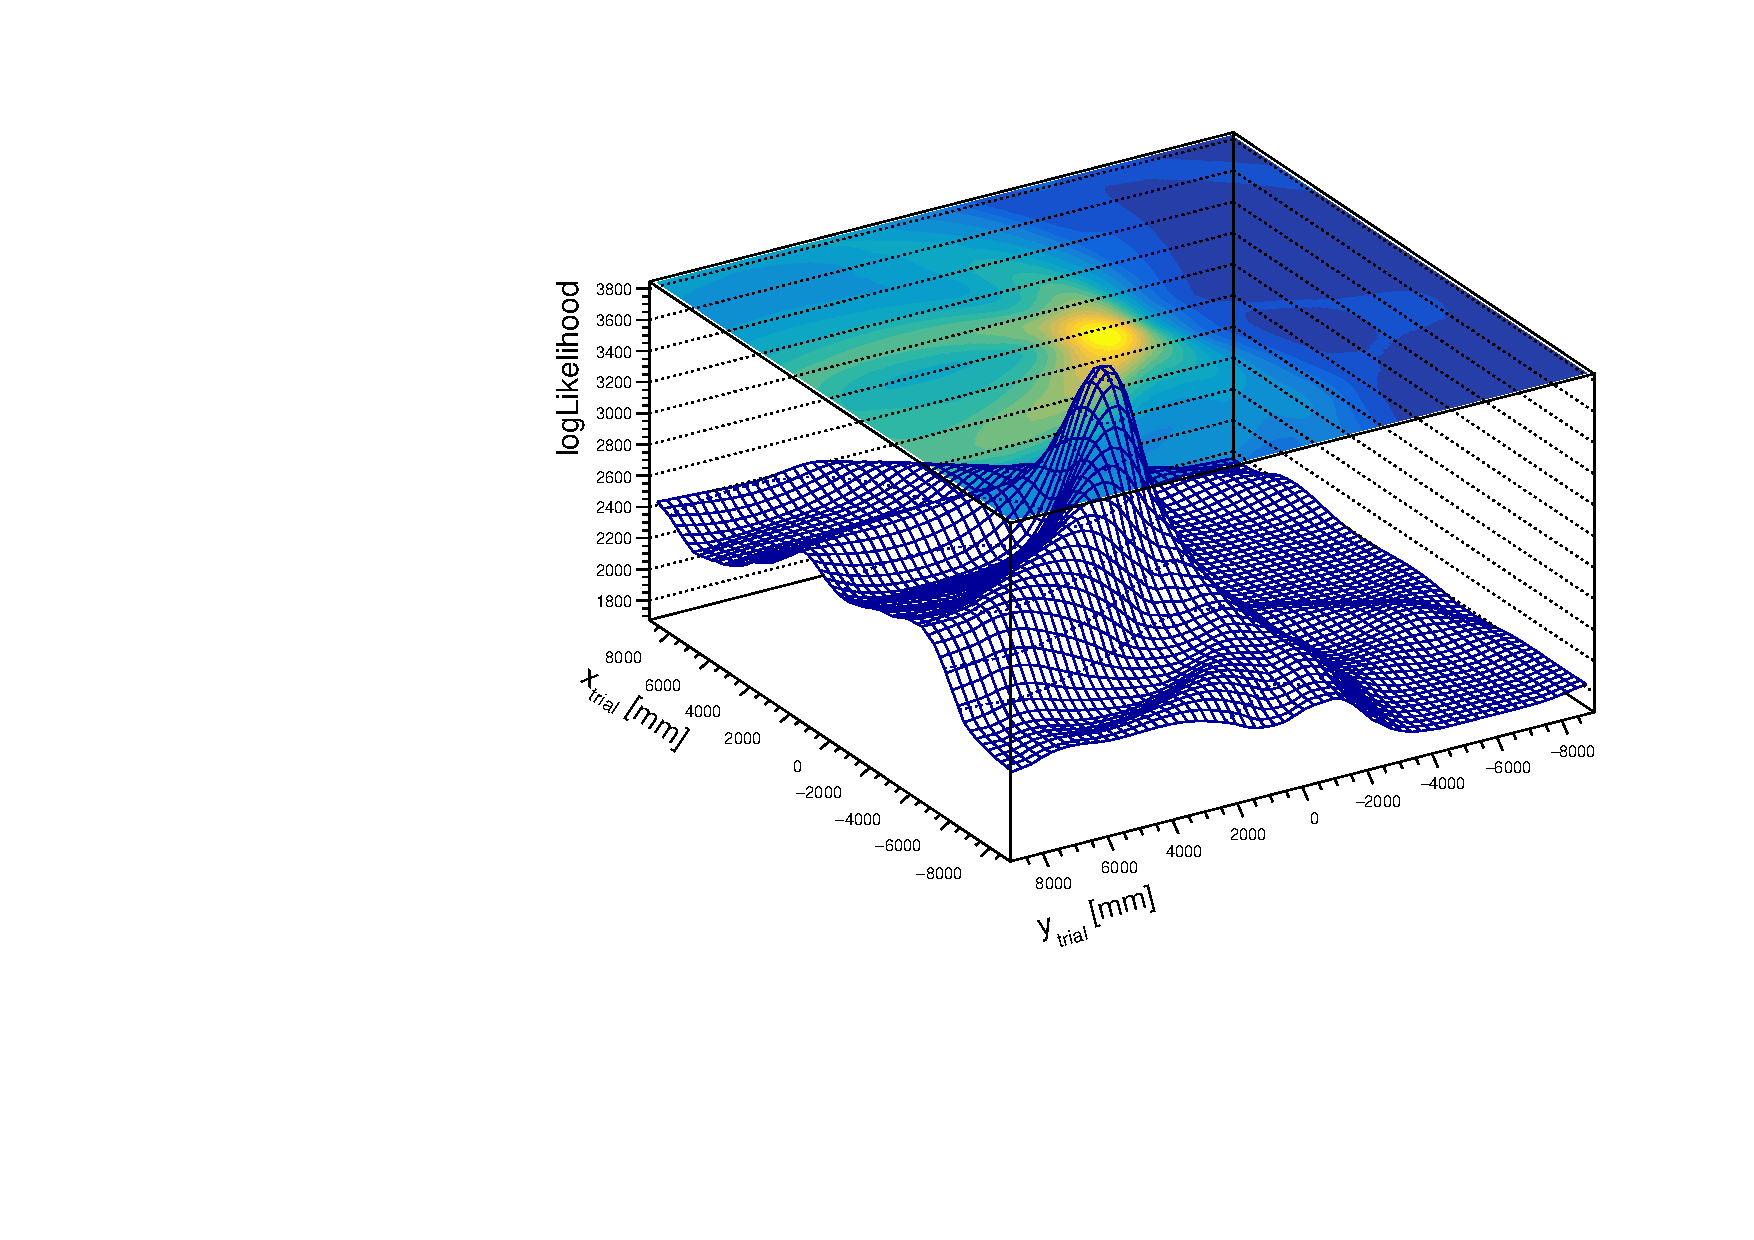
\includegraphics[width=75mm]{surf3_likelihoodXY.pdf}}
	\subfigure[Y-Z plane.]{\label{fig:1b}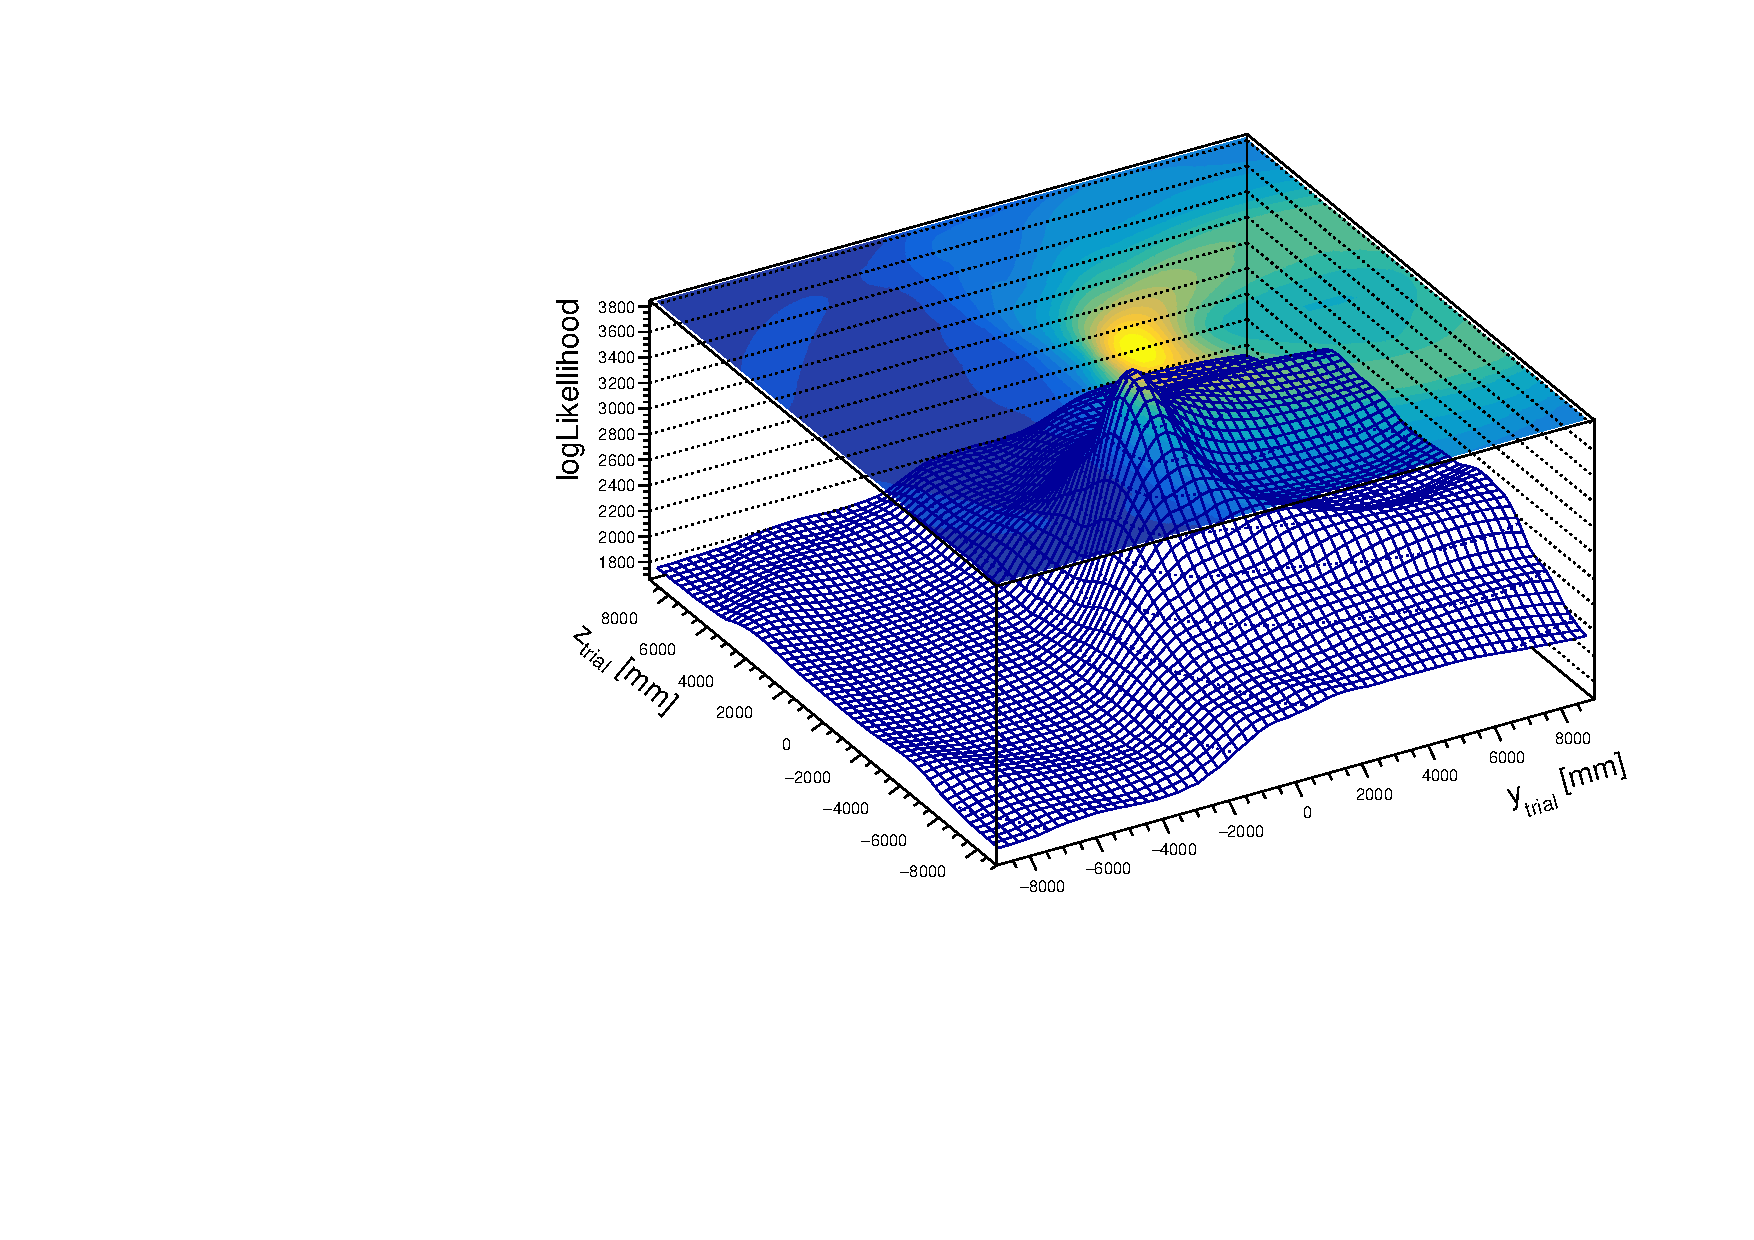
\includegraphics[width=75mm]{surf3_likelihoodYZ.pdf}}
	\subfigure[X-Z plane.]{\label{fig:1c}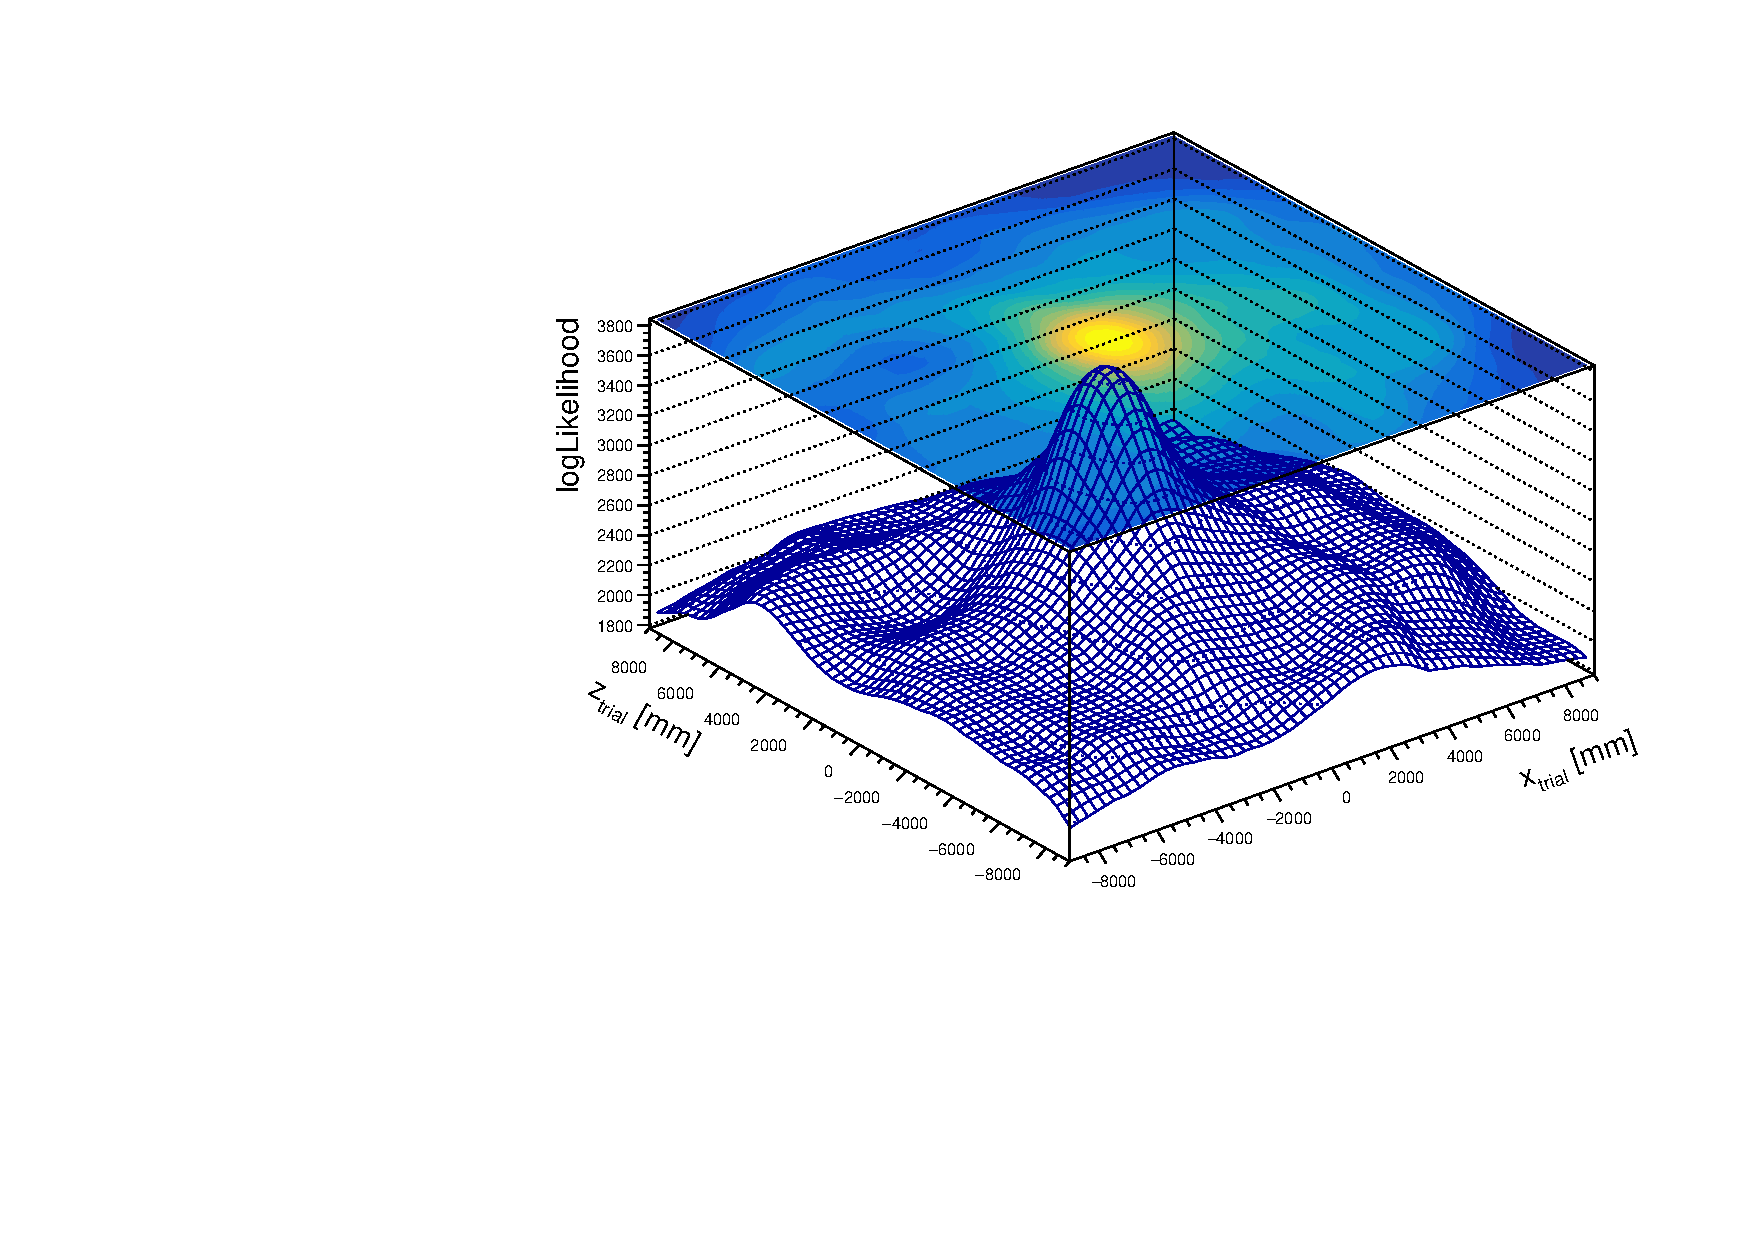
\includegraphics[width=75mm]{surf3_likelihoodXZ.pdf}}
	\caption{Likelihood surface of an {$^{16}$}N event projected on X-Y, Y-Z, X-Z planes. A clear global maxima is reached for the fitted vertex.}
	\label{likelihoodSurface}
\end{figure}


\begin{figure}
	\centering
	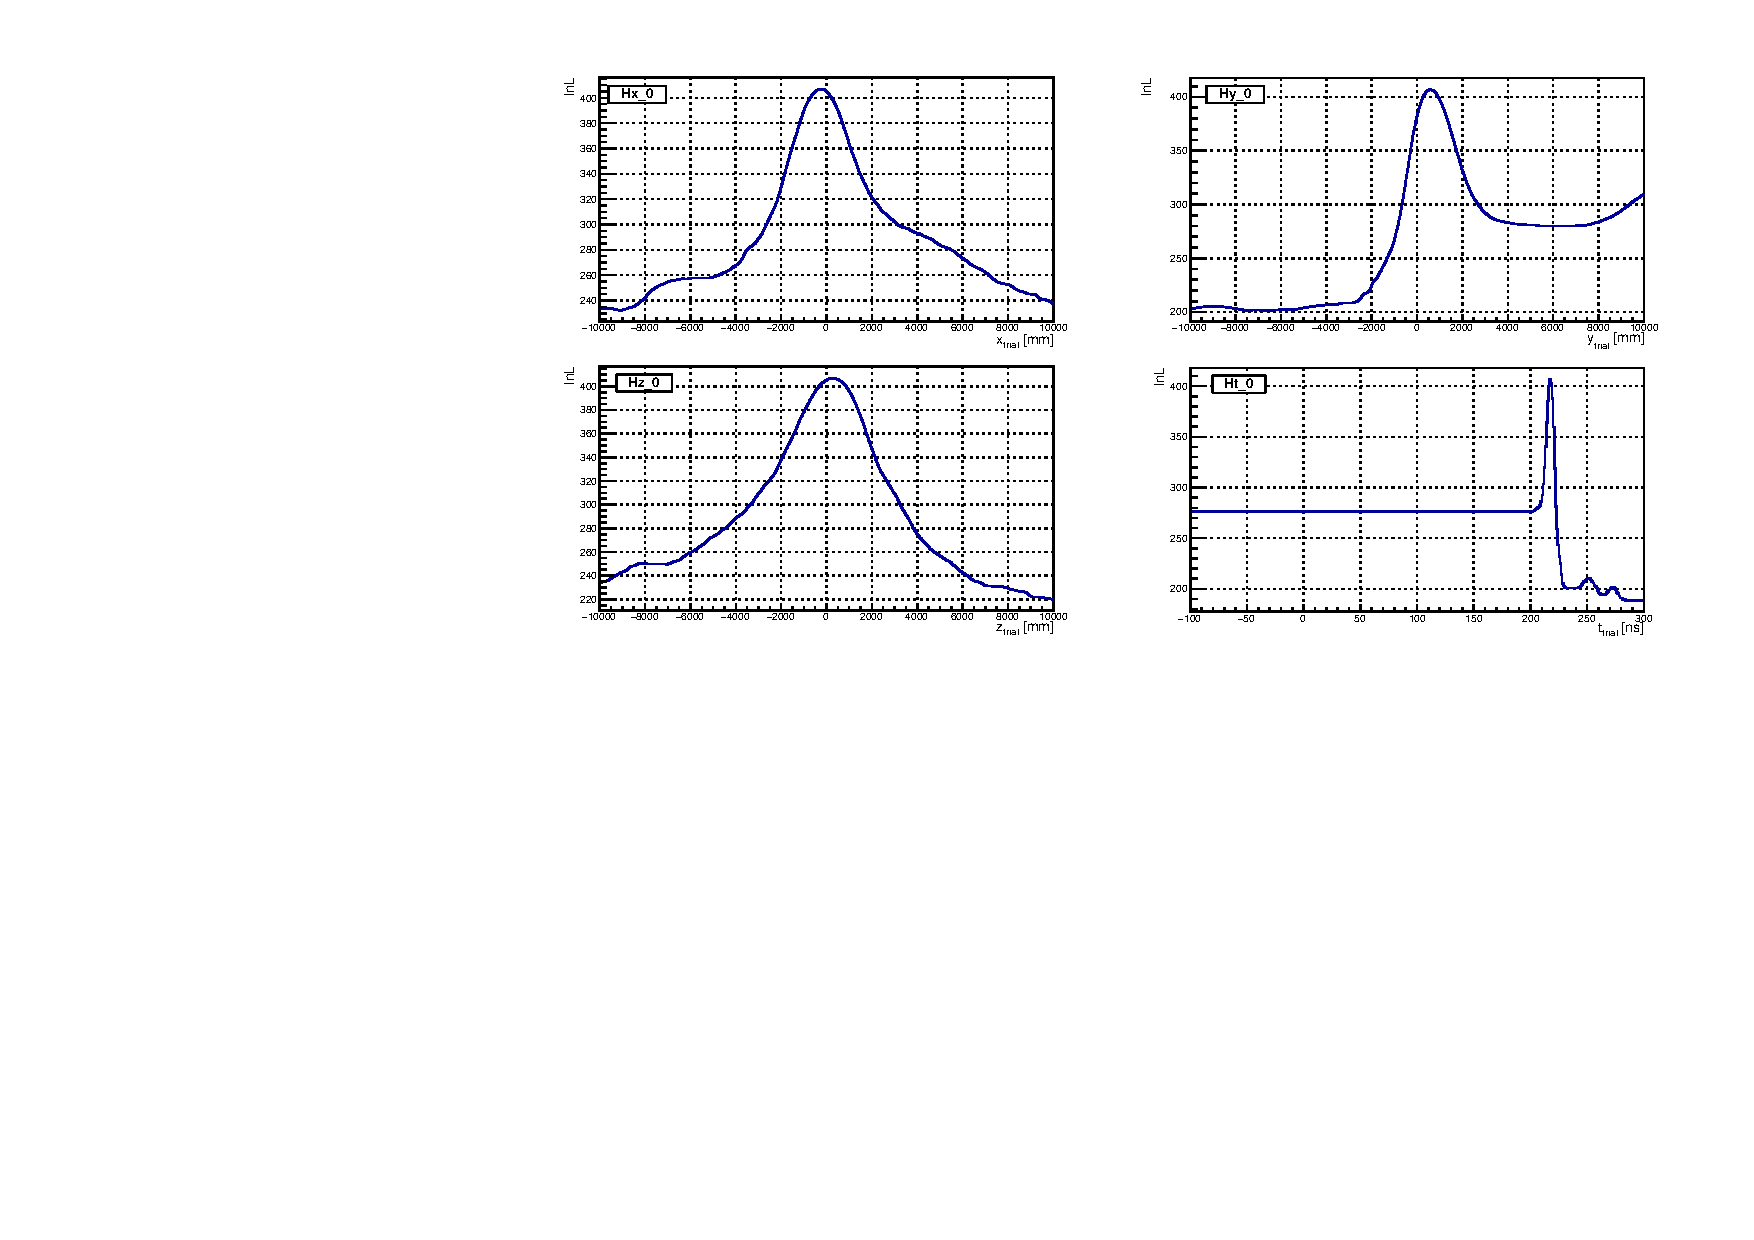
\includegraphics[width=160mm]{logL_xyzt.pdf}
	\caption{Likelihood surface of an {$^{16}$}N event projected on x, y, z, t axes.}
	\label{logLxyz}
\end{figure}

\begin{figure}
	\centering
	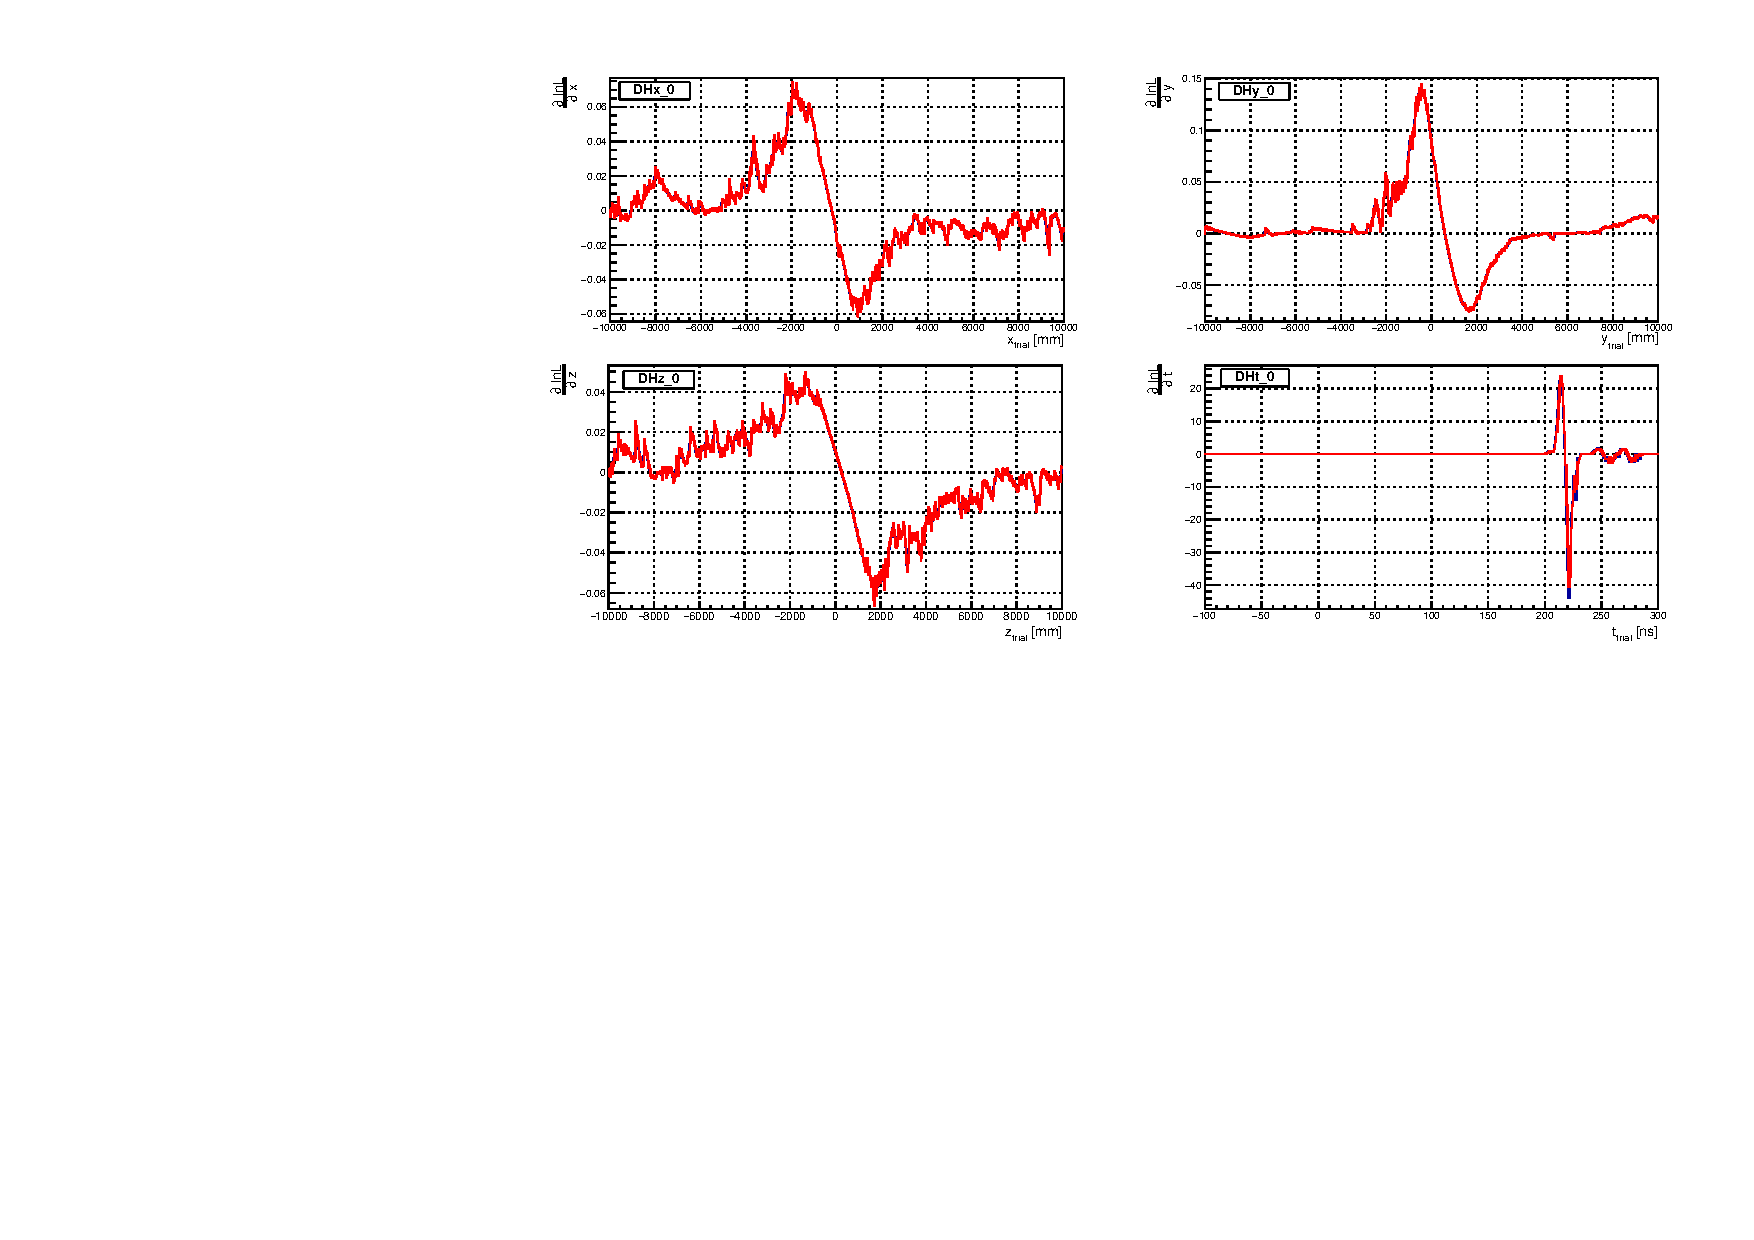
\includegraphics[width=160mm]{derivativeLogL_xyzt.pdf}
	\caption{Derivatives of logLikelihood of an {$^{16}$}N event projected on x, y, z, t axes. The analytical derivatives (blue) are overlaid with numerical derivatives (red). They are well-matched.}
	\label{derivative_logLxyz}
\end{figure}

emit $\gamma$-rays. These $\gamma$-rays will Compton scatter off electrons and the electrons will emit Cherenkov light to be detected by the PMTs.


\subsection{Angular Resolution}
An angular resolution function was 

It is defined as a combination of two exponential components:
\begin{equation}
P(\cos\theta)=\alpha_M\frac{\beta_M\exp[-\beta_M(1-\cos\theta)]}{1-\exp(-2\beta_M)}+(1-\alpha_M)\frac{\beta_s\exp[-\beta_s(1-\cos\theta)]}{1-\exp(-2\beta_s)},
\end{equation}
where the parameters: $\beta_M$ and $\beta_S$ are the ``decay'' constants or ``slopes'' of the two exponential components; the $\alpha_M$ is the fraction between two exponential components.
events following the exponential with slope βm. 


The angle θ is the displacement between the ‘truth’ and
reconstructed directions.

Direction resolutions, with a cut of $|\vec{X}_{fit}-\vec{X}_{src,manip}|>1.5~m$:

The fitted results are shown in Table.~\ref{angularResolValues}.
\begin{table}[ht]
	\begin{tabular}{cccccccc}%{|p{2.2cm}|p{1.8cm}|p{2cm}|p{2cm}|p{1.8cm}|p{1.1cm}|p{1.1cm}|p{1.1cm}| }
		\toprule
		107055& $\beta_M$ &  $\beta_S$ & $\alpha_M$ & $\chi^2$/ndf & $\cos\theta_{0.5}$ & $\cos\theta_{0.8}$& $\cos\theta_{0.9}$\\
		\hline
		Rat data & 3.50$\pm$0.11 & 18.48$\pm$0.82 & 0.51$\pm$0.02 & 127.8/140 & 0.991 & 0.733 & 0.338\\
		Rat MC  & 3.74$\pm$0.15 & 19.58$\pm$0.92 & 0.48$\pm$0.02 & 137.1/138 & 1 & 0.768 & 0.398\\	
		\hline
		MPW data & 3.79$\pm$0.12 & 18.58$\pm$0.95 & 0.53$\pm$0.02 & 154.6/143 & 0.982 & 0.743 & 0.379\\
		MPW MC &4.01$\pm$0.19 & 18.41$\pm$1.06 & 0.48$\pm$0.03 & 128.4/127 & 1 & 0.779 & 0.433  \\
		\bottomrule
	\end{tabular}
	\label{angularResolValues}
\end{table}


Fig.~\ref{angularResolMPW} shows the fits of the angular distributions after $|\vec{X}_{fit}-\vec{X}_{src,manip}|>1.5~m$ cuts.
\begin{figure}
	\centering
	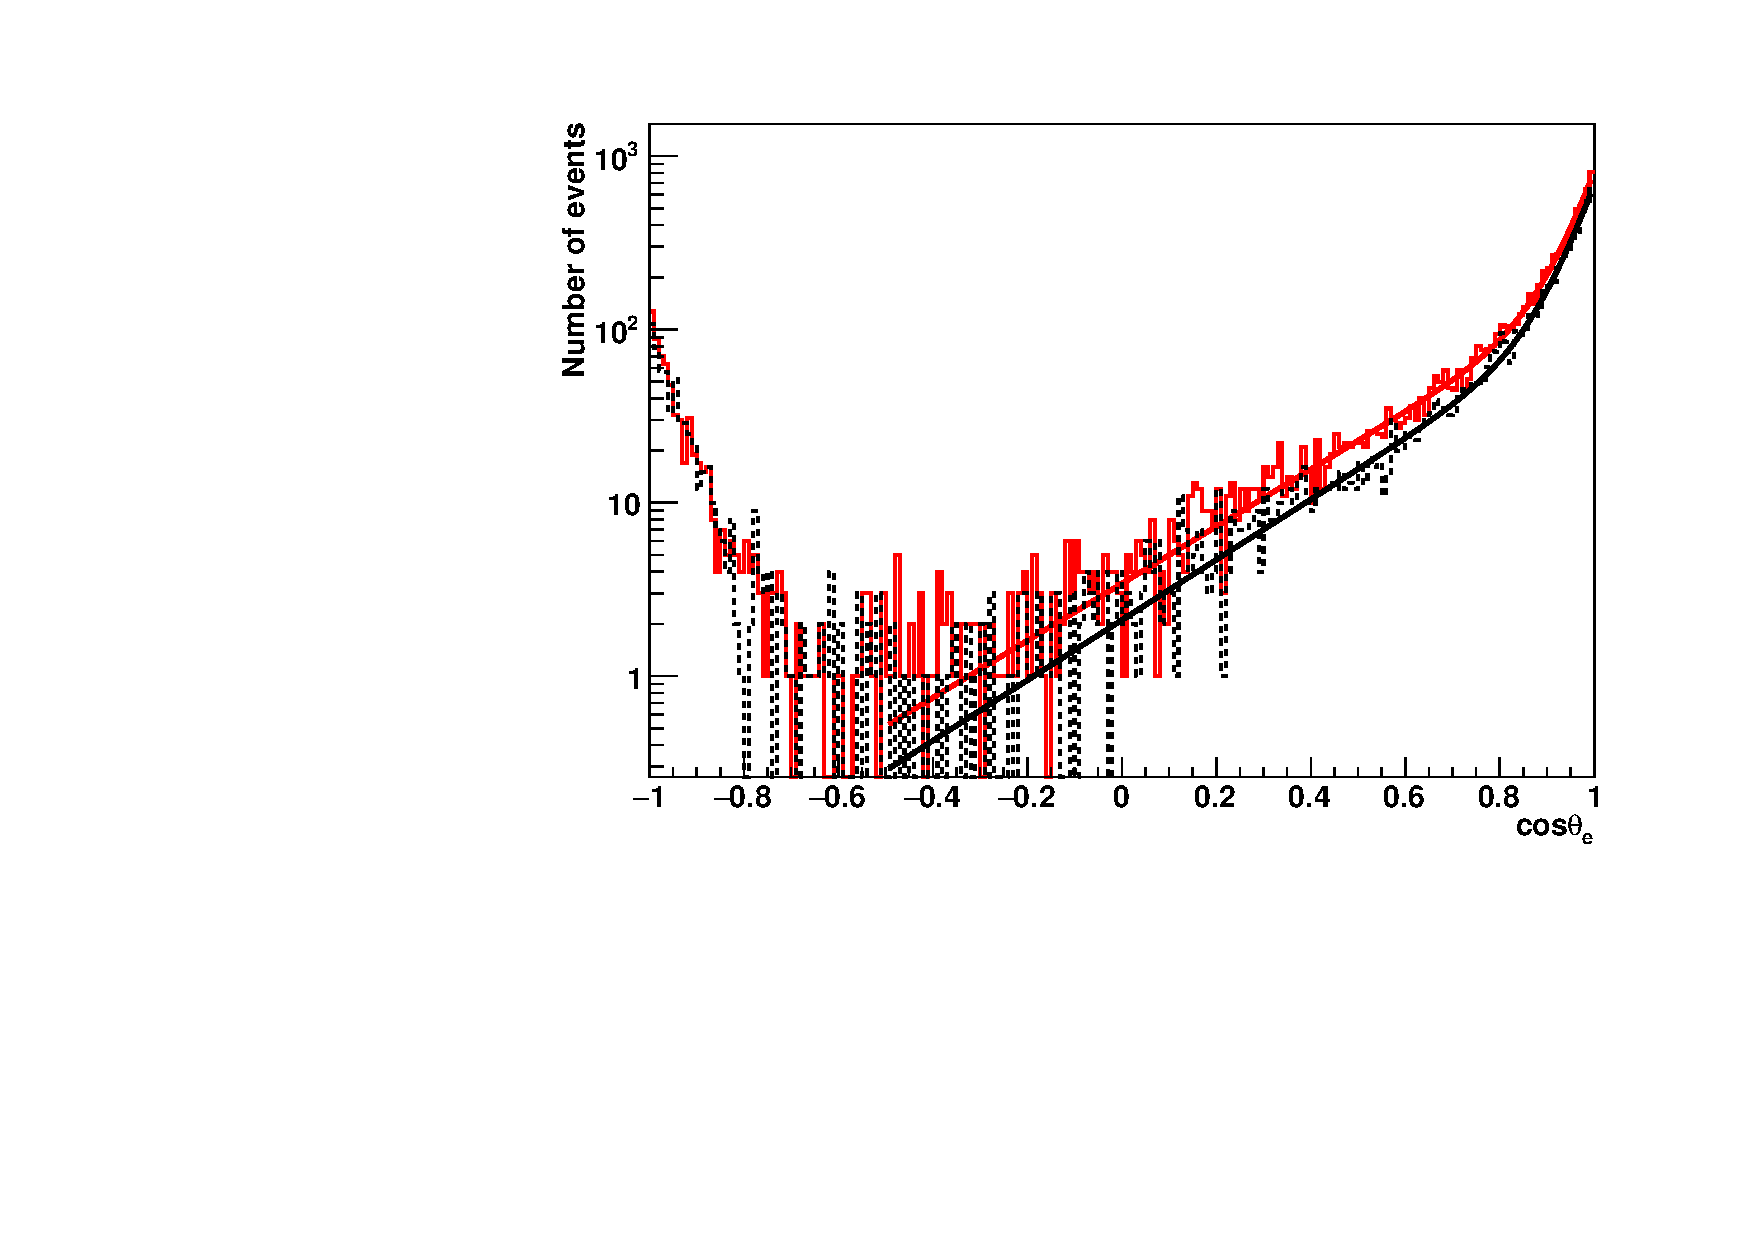
\includegraphics[width=8cm]{angularResol_107055_mpw.pdf}
	\caption{Angular distributions fitted with angular resolution functions, compared the data (red solid line) with the MC (black dashed line).}
	\label{angularResolMPW}
\end{figure}

To describe the $\cos\theta_e$ distribution, the angles that contain 50\%, 80\%
and 90\% of the reconstructed events, the $\cos\theta_{0.5}$, $\cos\theta_{0.8}$ and $\cos\theta_{0.9}$ can also be used. Their values are solved numerically by the equation \ref{eq:cosTheta_e} below (take $\cos\theta_{0.5}$ as an example):

\begin{equation}\label{eq:cosTheta_e}
\frac{\int_{\cos\theta_{0.5}}^1 P(\cos\theta_e) d\cos\theta_e}{\int_{-1}^1 P(\cos\theta_e) d\cos\theta_e} = 50\%,
\end{equation}

where $P(\cos\theta_e)$ is the direction resolution function with the best fitted parameters. If these values are large, the $\cos\theta_e$ distribution is sharper and more peaked around +1.

\section{Energy}

The reconstructed energy of the $^{16}$N events are shown in Fig.~\ref{N16energy}. The results from the MC and the data are compared.
\begin{figure}[htbp]
	\centering
	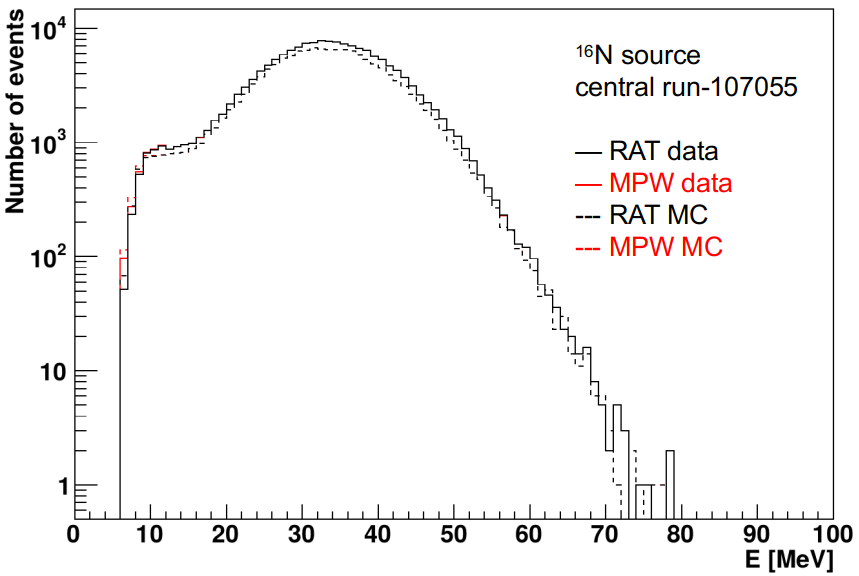
\includegraphics[width=8cm]{N16_nhits_107055.png}
	\caption{NHit spectrum for the $^{16}$N central run-107055. Dashed lines for the MC and solid lines for data; red for the MPW fitter results and black for the Rat results.}
	\label{N16nhits}
\end{figure}



\begin{figure}[htbp]
	\centering
	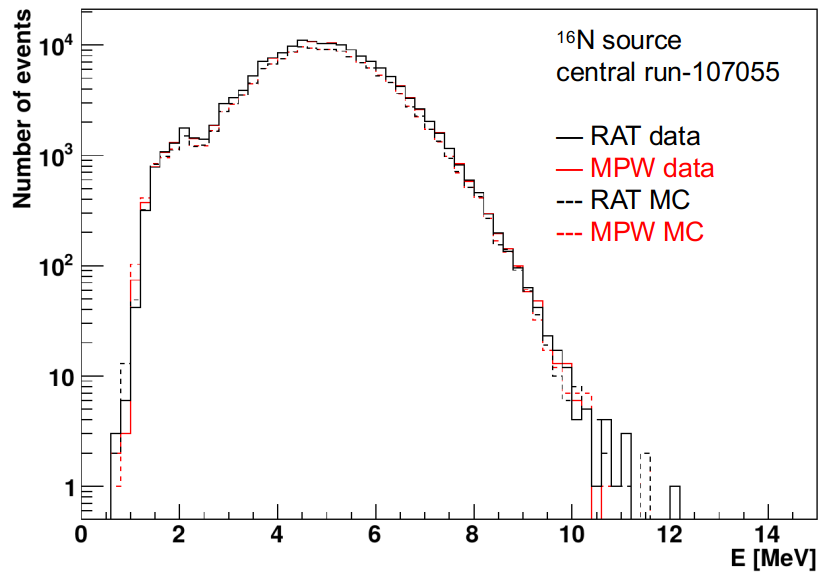
\includegraphics[width=8cm]{N16_reconE_107055.png}
	\caption{Reconstructed energy spectrum for the $^{16}$N central run-107055. Dashed lines for the MC and solid lines for data; red for the MPW fitter results and black for the Rat results.}
	\label{N16energy}
\end{figure}

\begin{figure}[htbp]
	\centering
	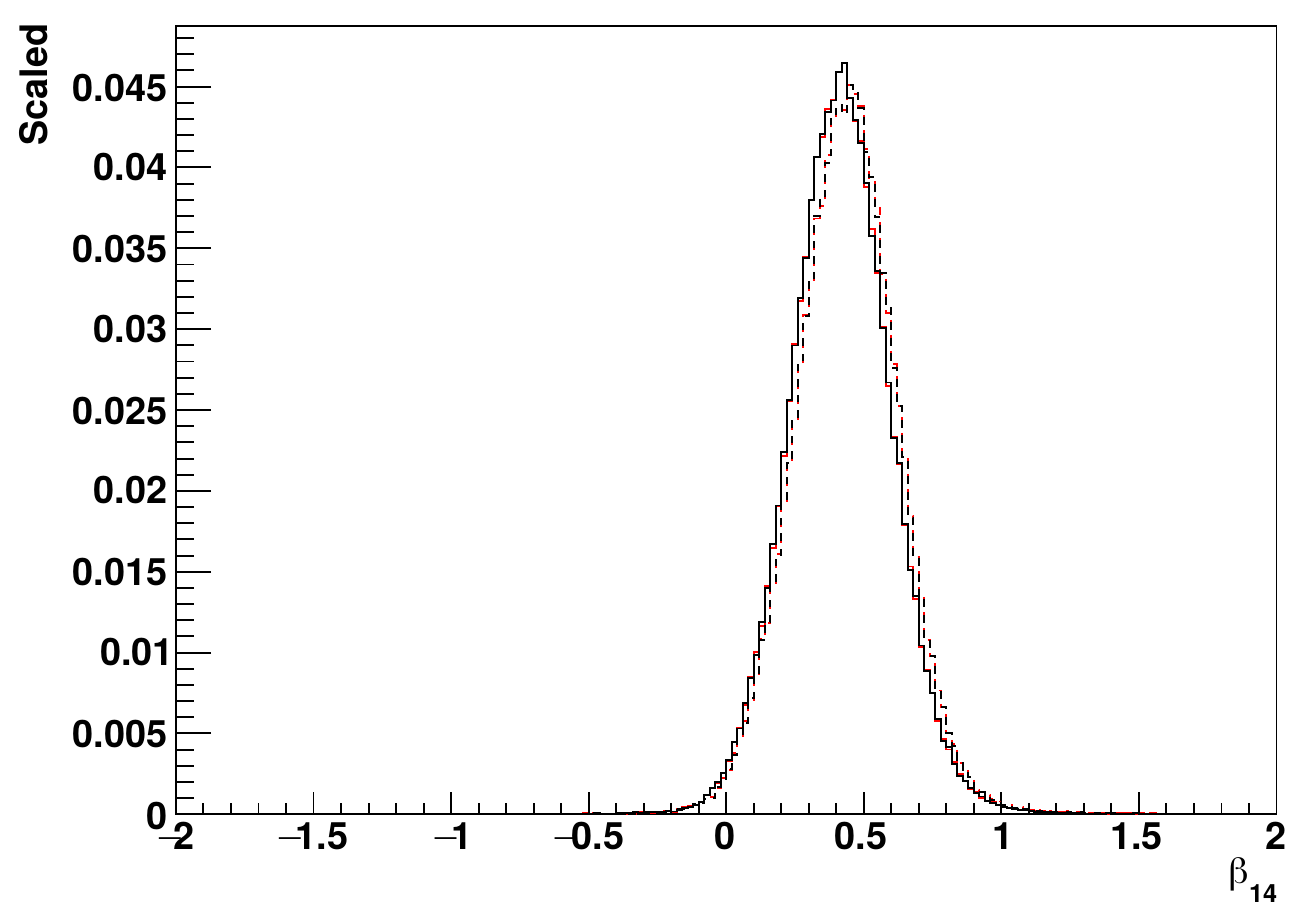
\includegraphics[width=8cm]{N16_beta14_107055.png}
	\caption{Distributions of $\beta_{14}$ for the $^{16}$N central run-107055. Dashed lines for the MC and solid lines for data; red for the MPW fitter processed results and black for the Rat results.}
	\label{N16beta14}
\end{figure}


\begin{figure}[htbp]
	\centering
	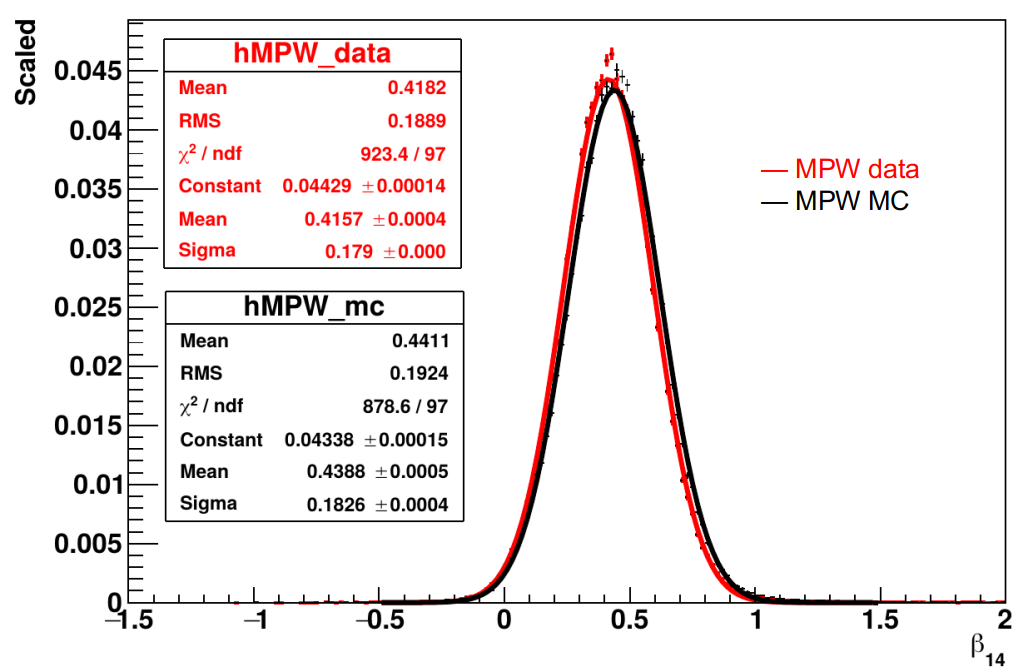
\includegraphics[width=8cm]{N16FitMPW_beta14_107055.png}
	\caption{Comparisons of the $\beta_{14}$ for the data and the MC. Both of the distributions are the MPW processed results and are fitted with Gaussian distributions in a region of $[-0.5,1.5]$. The data shows a smaller mean value (0.4157) than the MC (0.4388).}
	\label{N16beta14MPW}
\end{figure}



\section{Extracting \texorpdfstring{$\gamma$}{Lg}-rays from Neutron Capture}
The AmBe calibration source is used for the calibrations of the SNO+ neutron capture process.


\section{Solar \texorpdfstring{$\nu_e$}{Lg} Analysis and Background Separation in Water Phase}


solar neutrino candidate events in the open dataset.

\begin{figure}[htbp]
	\centering
	\subfigure[Run 100093, GTID 11108354]{ 
		\begin{minipage}[t]{0.4\textwidth}
			\centering
			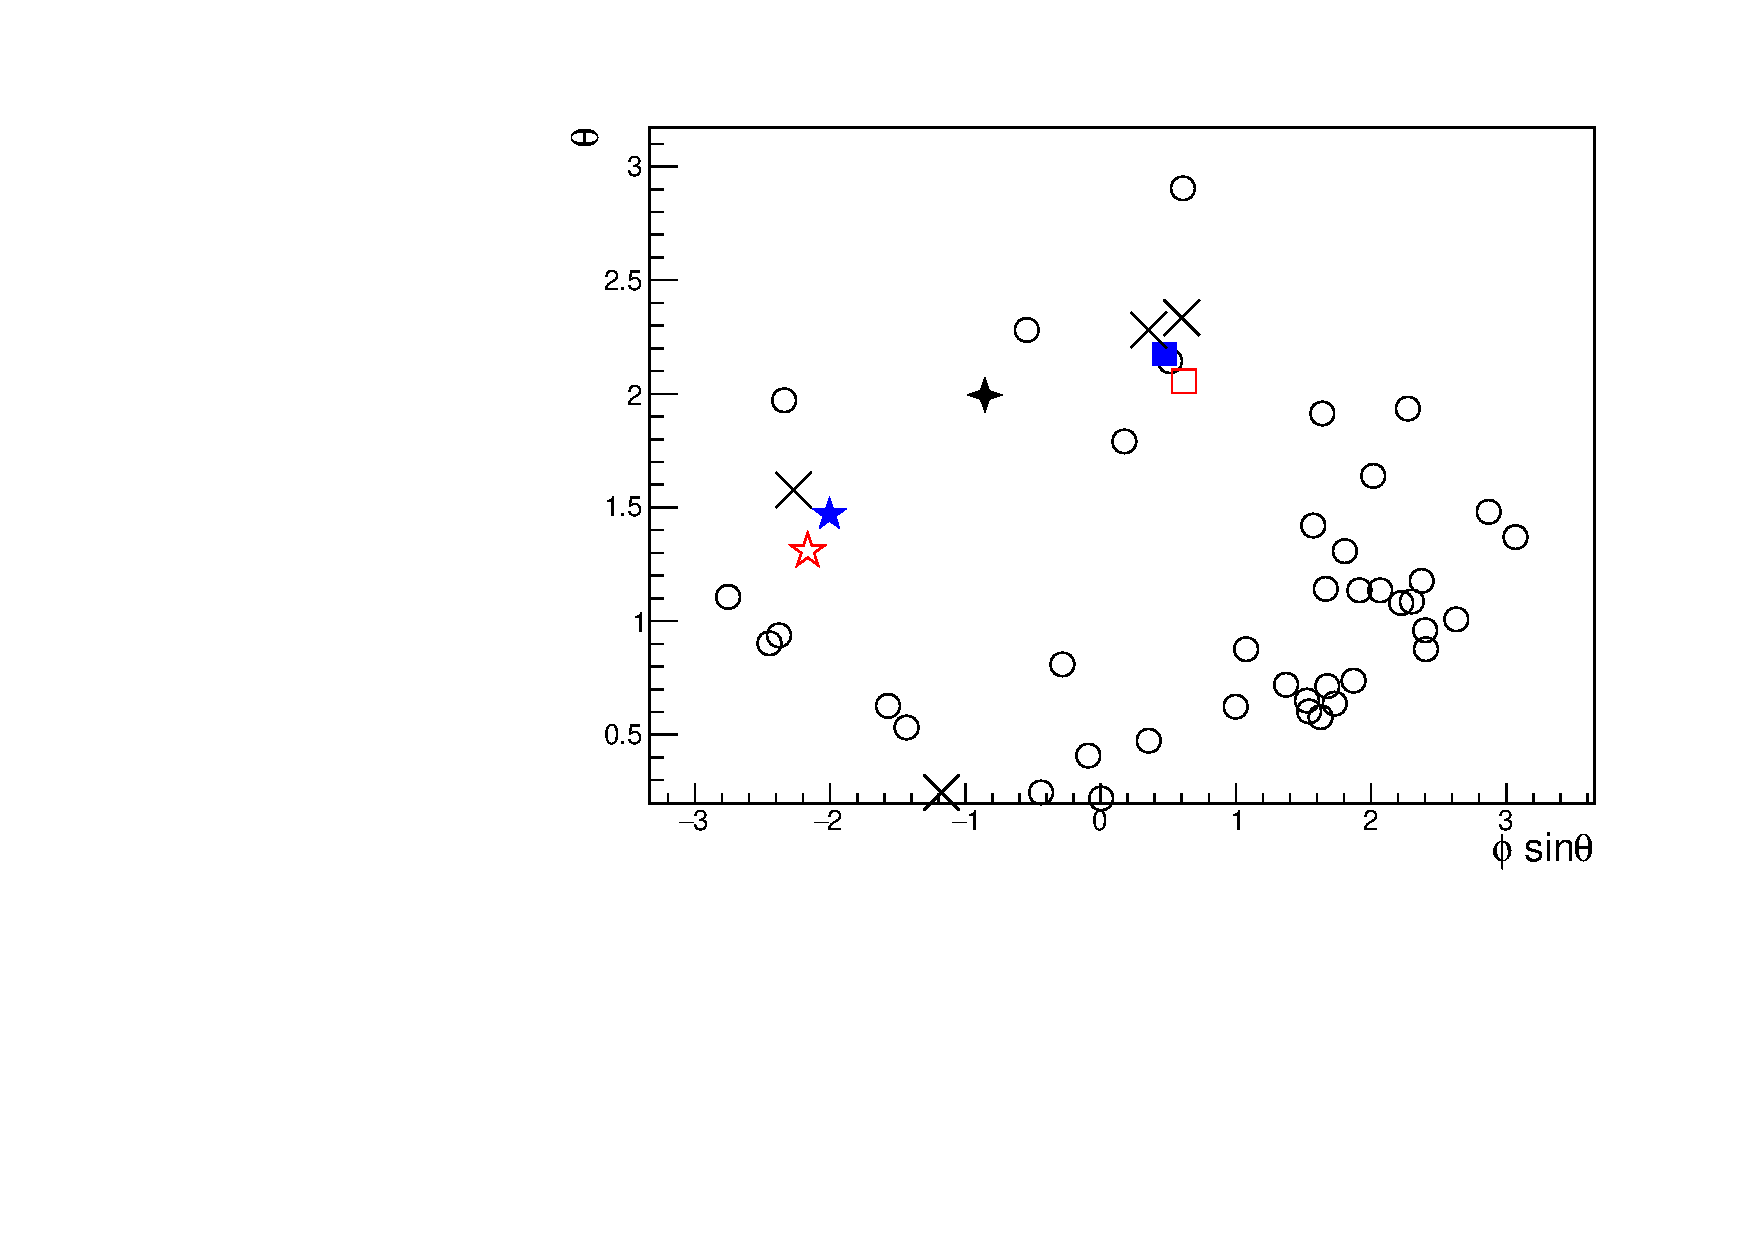
\includegraphics[width=6cm]{PMTmap_100093.pdf}
		\end{minipage}
	}
	\subfigure[Run 100207, GTID 5079885]{ 
		\begin{minipage}[b]{0.4\textwidth}
			\centering
			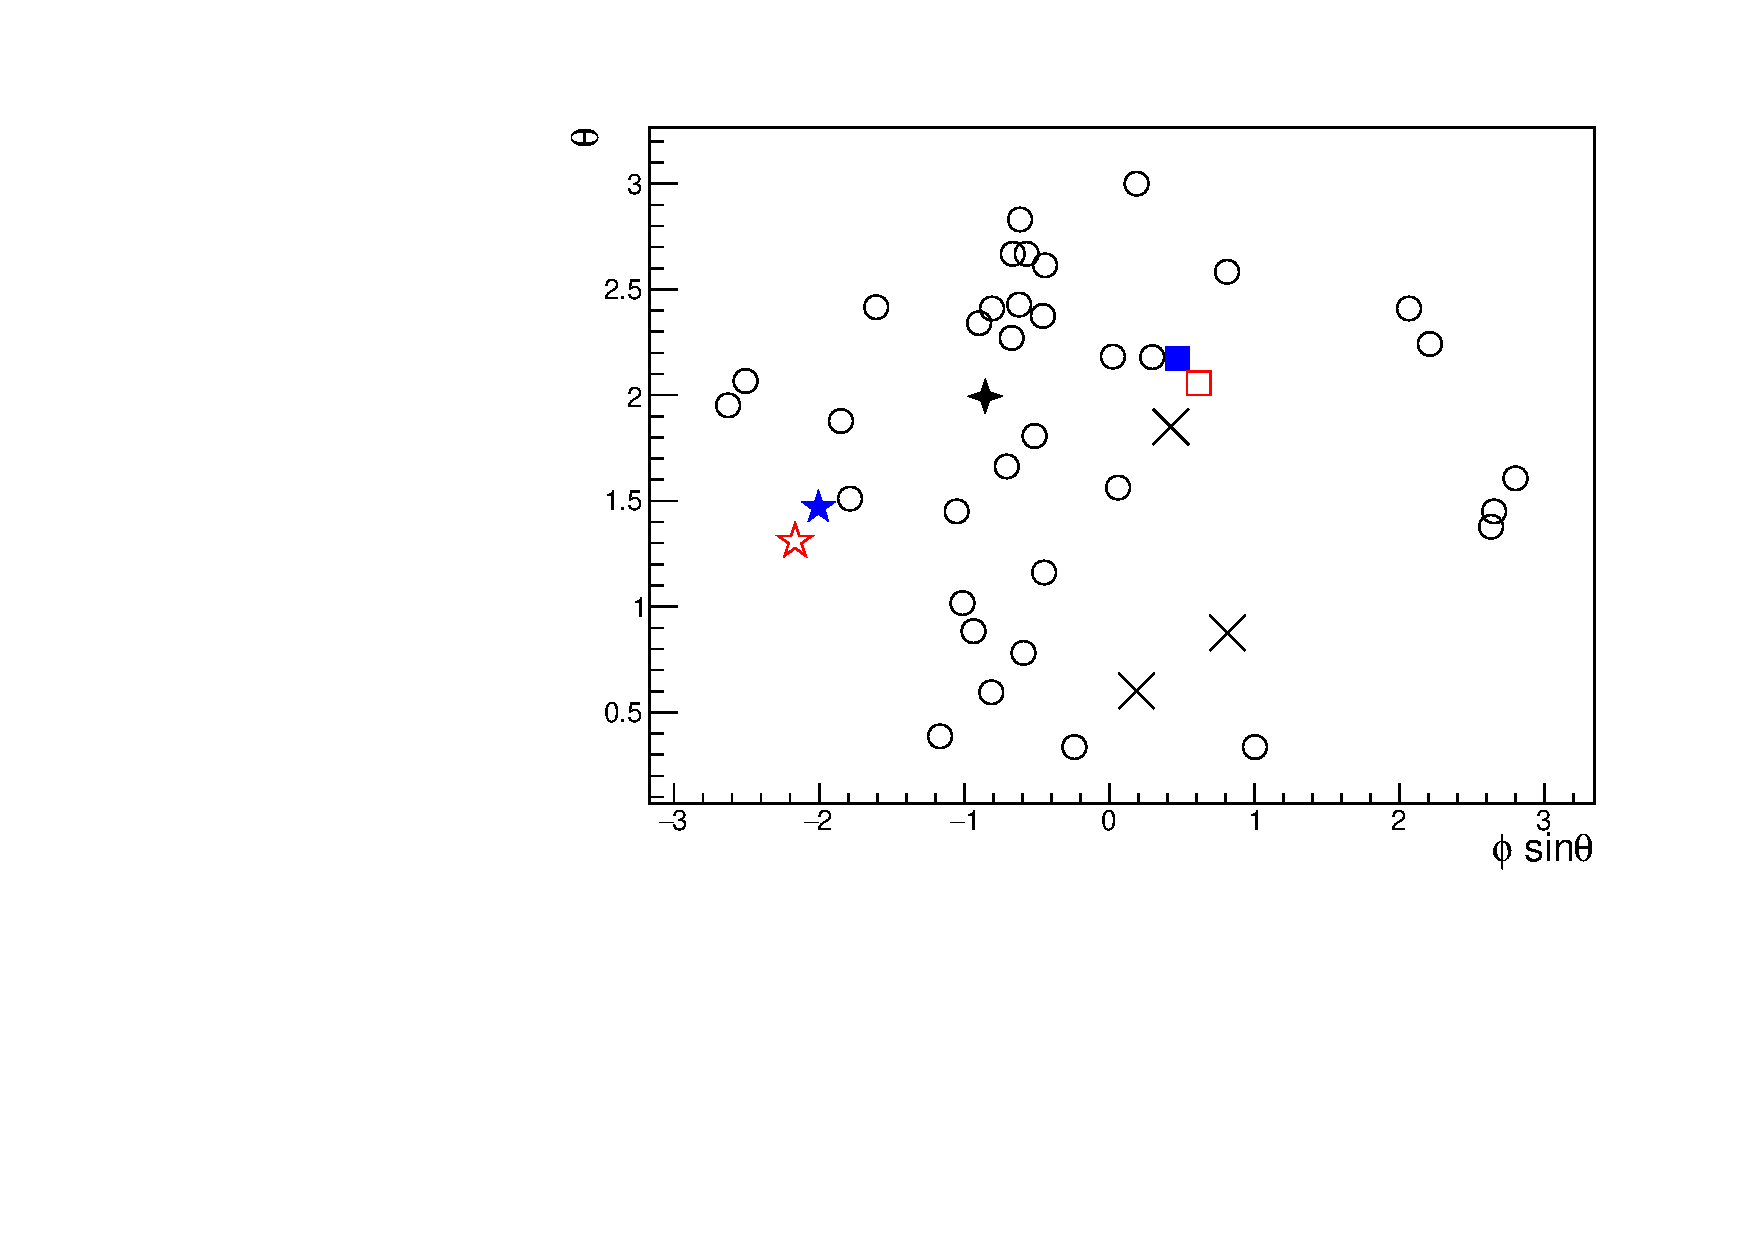
\includegraphics[width=6cm]{PMTmap_100207.pdf}
		\end{minipage}
	}
	\subfigure[Run 100632, GTID 7882360]{ 
		\begin{minipage}[t]{0.4\textwidth}
			\centering
			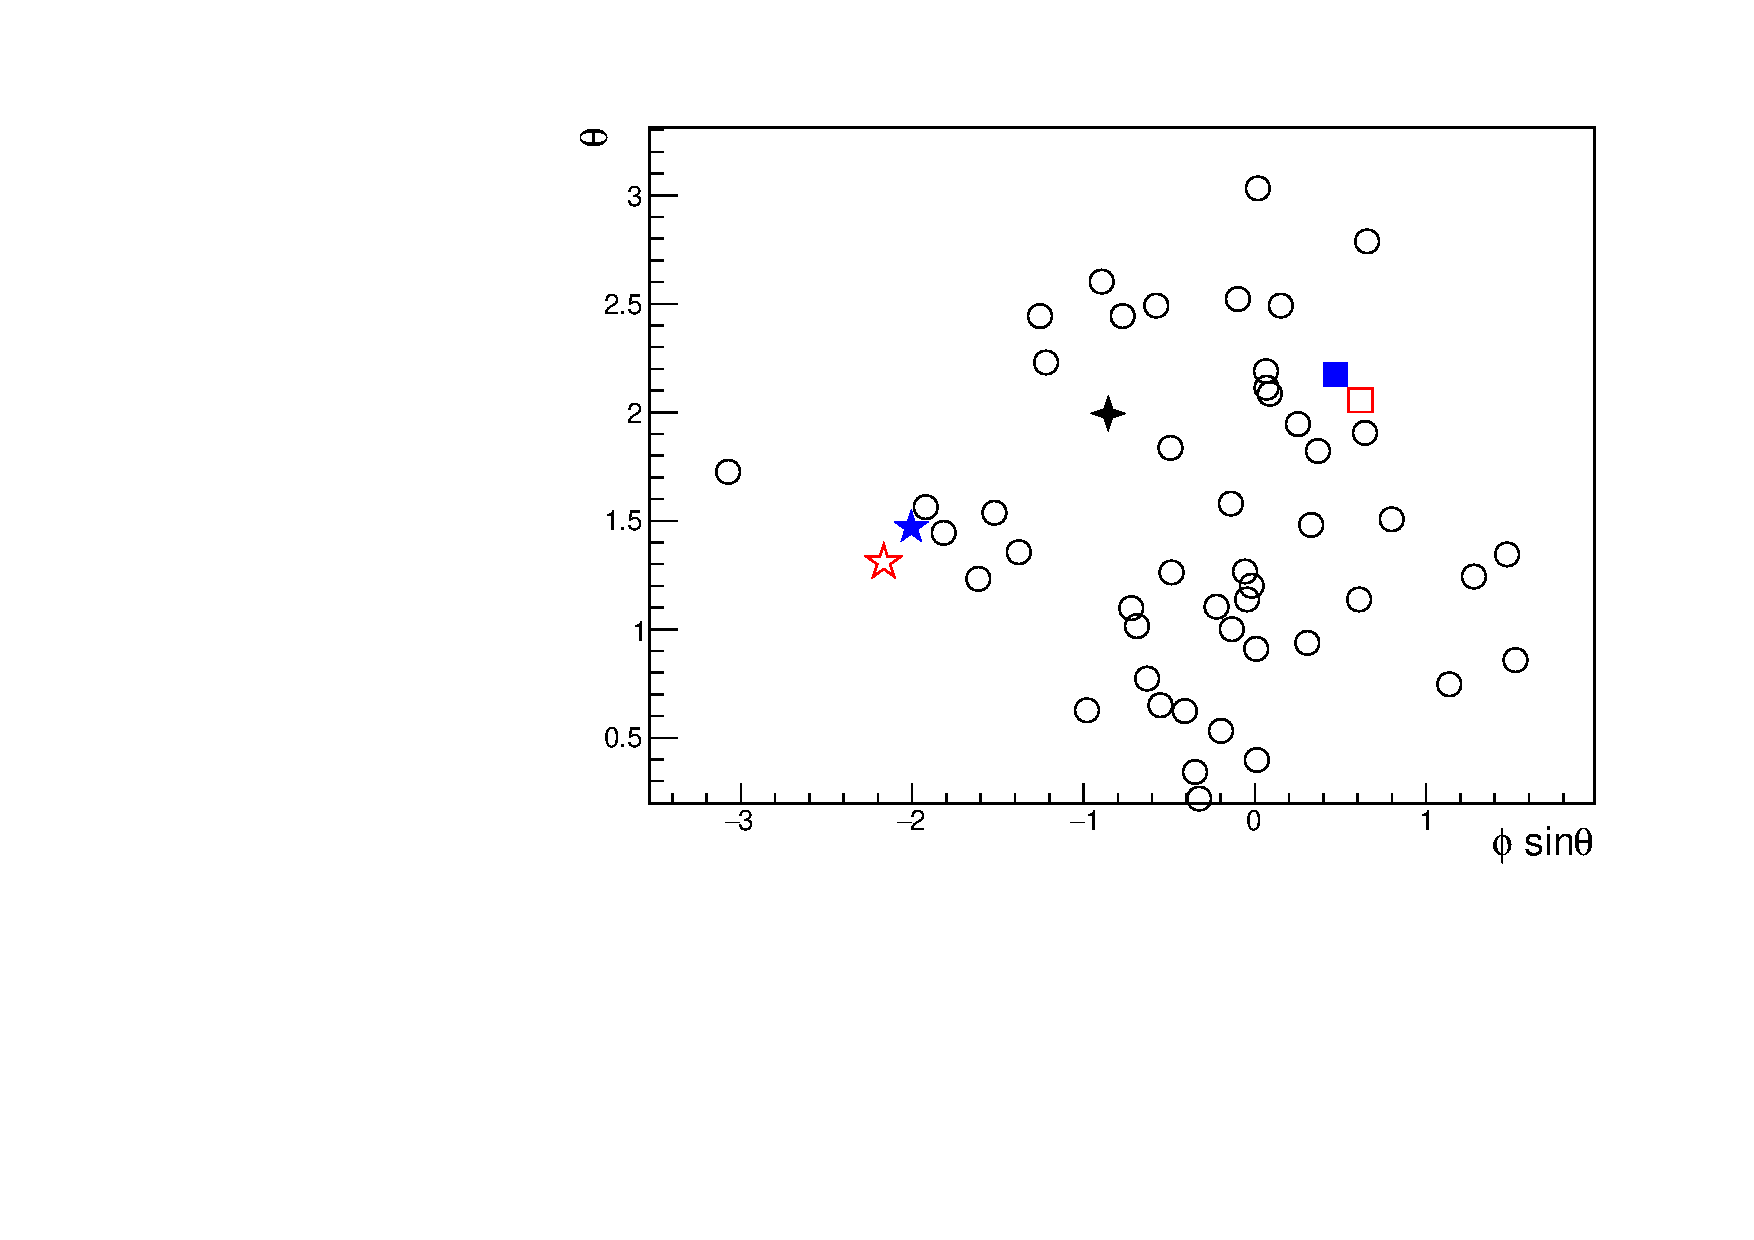
\includegraphics[width=6cm]{PMTmap_100632.pdf}
		\end{minipage}
	}
	\subfigure[Run 100663, GTID 15767175]{ 
		\begin{minipage}[t]{0.4\textwidth}
			\centering
			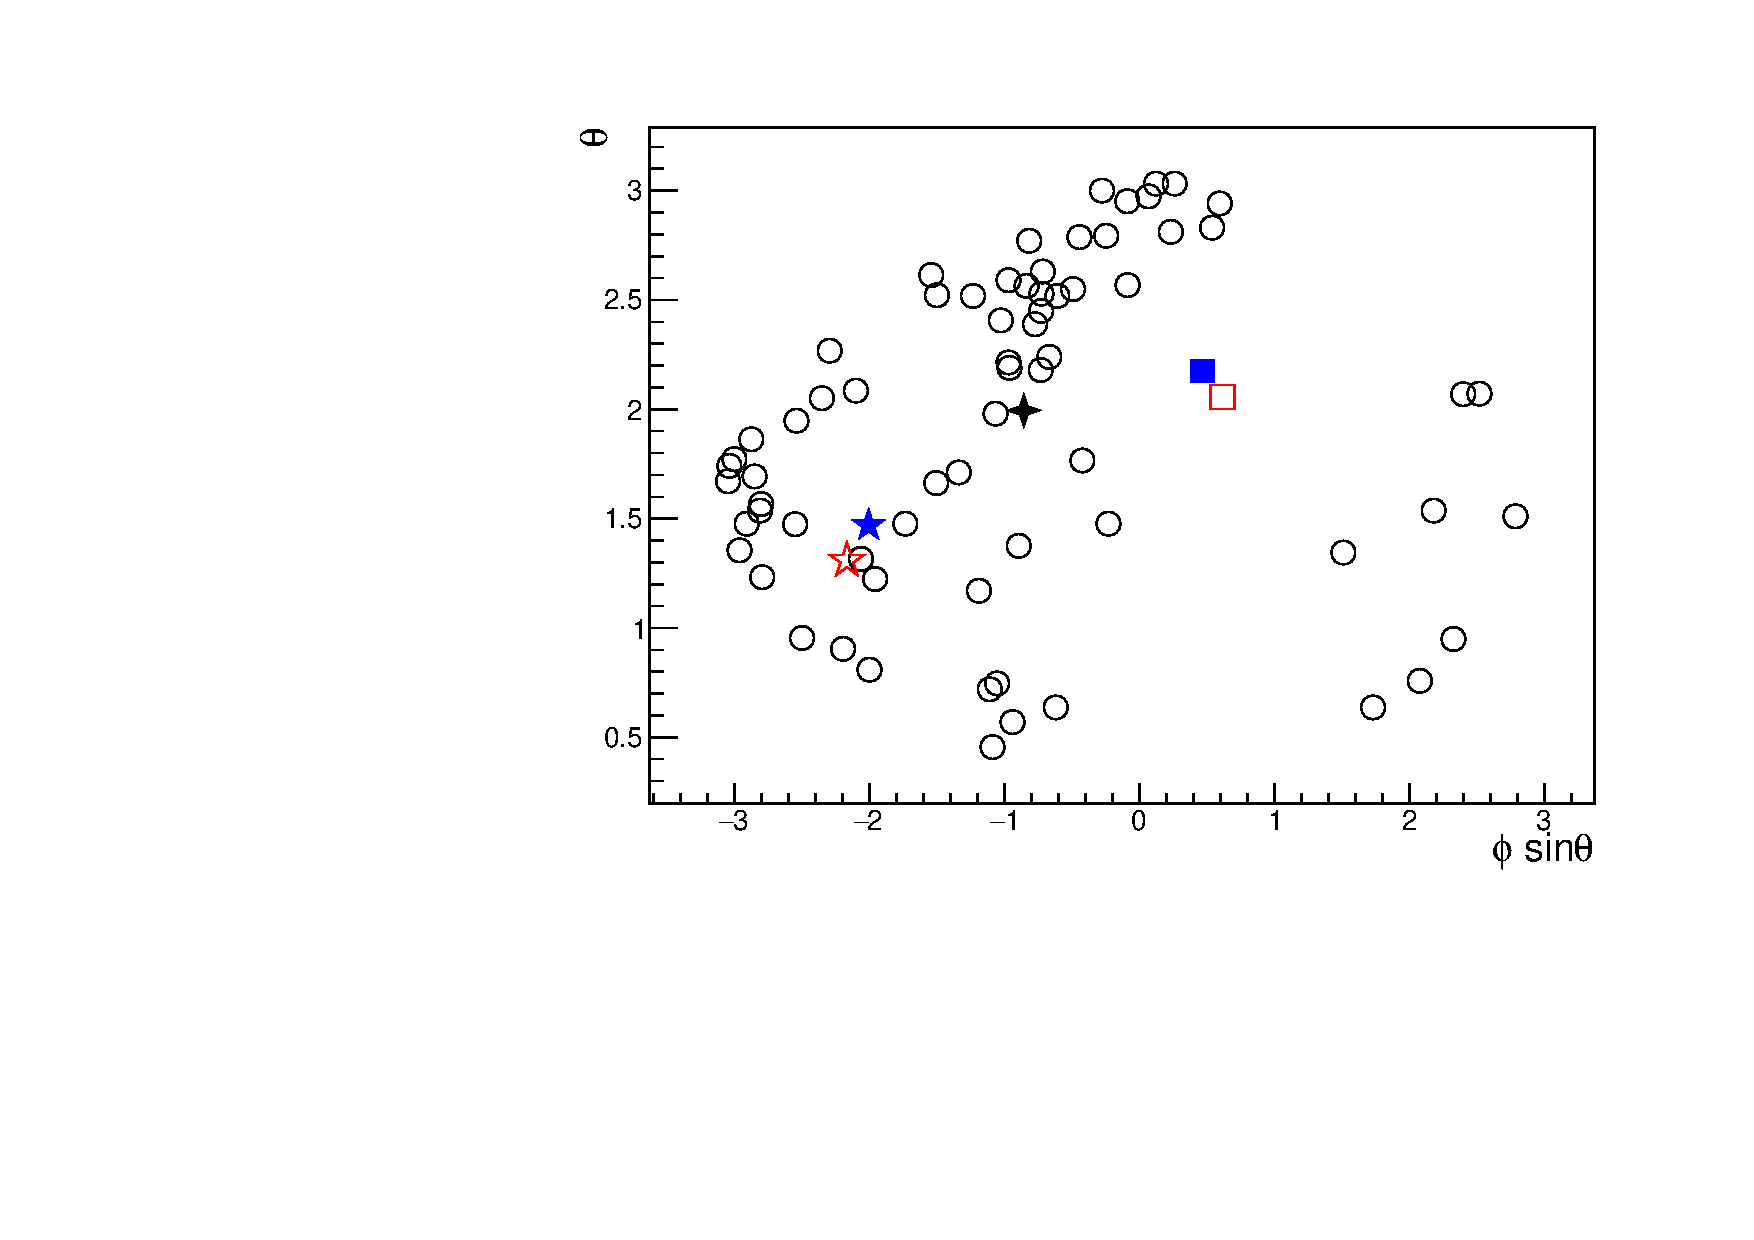
\includegraphics[width=6cm]{PMTmap_100663.pdf}
		\end{minipage}
	}
	\subfigure[Run 100915, GTID 169700]{ 
	\begin{minipage}[t]{0.4\textwidth}
		\centering
		{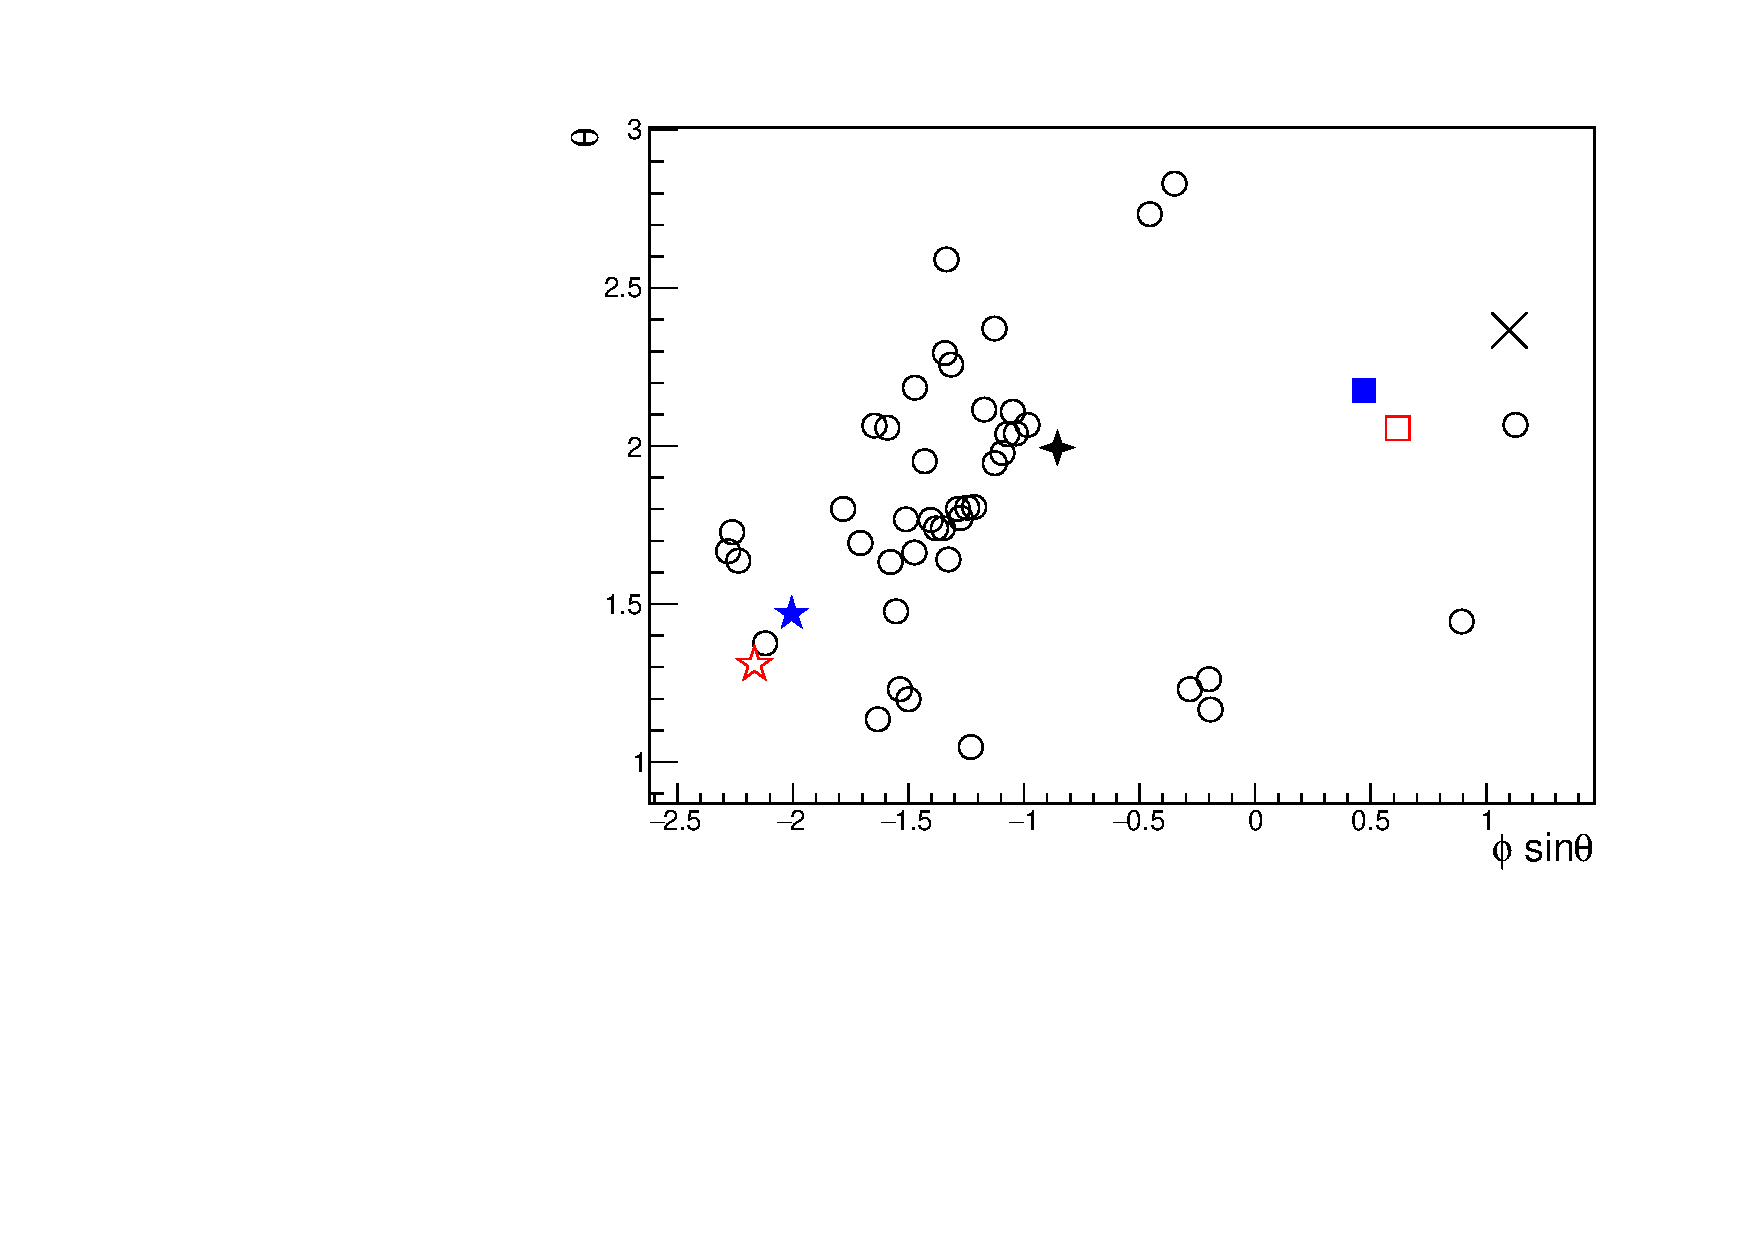
\includegraphics[width=6cm]{PMTmap_100915.pdf}}
	\end{minipage}
    }
	\subfigure[Legends]{ 
	\begin{minipage}[b]{0.4\textwidth}
		\centering
		{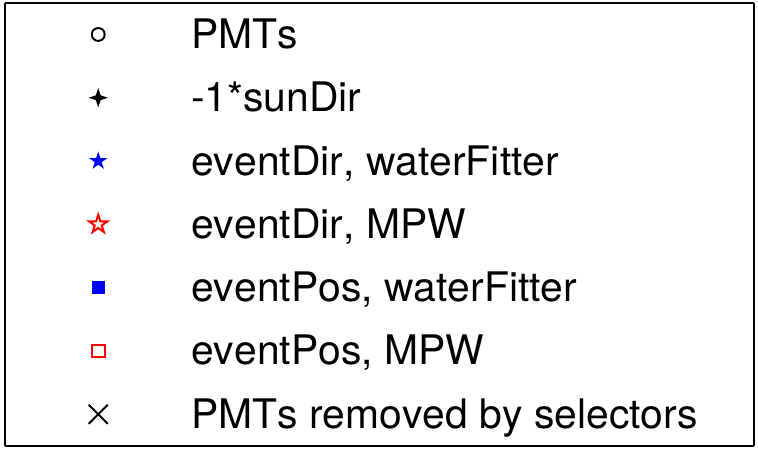
\includegraphics[width=5cm]{solarLegends.png}}
	\end{minipage}
    }
	\caption{Fit results for the candidate events, projected onto PMT sinusoidal maps. Black circles stand for
	the hit PMTs used by the fitter; crosses stand for the hit PMTs removed by the selectors; blue full star stands for the event direction fitted by the waterFitter; red open star stands for the direction fitted by the MPW; full double diamond stands for the solar direction*-1; blue full square stands for the event position fitted by the waterFitter; open square stands for the position fitted by the MPW.}
	\label{openDataSetCandidate}
\end{figure}











The Toolkit for Multivariate Data Analysis with ROOT (TMVA) \cite{tmvaWebsite}

TMVA 


other packages developed for high energy particle physics, such as StatPatternRecognition (SPR)\cite{sprWebsite}, can be considered as an alternative tool or as a reference for results comparisons. 

\subsubsection{Open Dataset Analysis}

MPW fit results

fiducial volume cut






\begin{table}[ht]
	\centering
	\caption{Candidate events in the open dataset. Compared the fitted results of the candidate events with different fitters.}
	\label{opendata}
	\begin{tabular*}{150mm}{c@{\extracolsep{\fill}}cccccccc}
		\toprule
	 Fitter &	Run &  GTID &  $z-0.108$(m) & $R$(m)& $(R/R_{av})^3$ & $\cos\theta_{sun}$ & SNO+ Day\\
		\hline 
	Rat & 100093 &11108354 &3.49 &3.57 &0.21 &-0.954459 &2683.92 \\	
	MPW &  --& --& 3.43 &	3.52 &	0.20	& -0.906388 & --\\
	Rat &	100207 &5079885 &-2.61 &4.60 &0.45 &0.816215 &2687.04\\
	MPW &	 --& --& -3.63 & \textbf{7.61} &	2.03 & \textbf{0.656374} & -- \\
	Rat &100632 &7882360 &1.77 &3.19 &0.15 &0.937212 &2696.93\\
	 MPW &    --& --&  1.67 & 3.11 &	0.14 & 0.910527 & -- \\
	Rat &100663 &15767175 &-4.33& 4.96 &0.56 &0.977517 &2698.18\\
	MPW & --& -- &-4.45 &	5.07 &	0.60 &	0.979943 & -- \\
	Rat &100915 &169700 &-1.00 &5.10 &0.61 &0.341287 &2701.23\\
	MPW &	--& --& -1.08 &	5.08 &	0.61 &	0.336706 & -- \\	
		\bottomrule
	\end{tabular*}
\end{table}


\begin{table}[ht]
	\centering
	\caption{Candidate events in the open dataset, searched by the MPW fitter.}
	\label{opendataMPW}
	\begin{tabular*}{150mm}{c@{\extracolsep{\fill}}cccccccc}
		\toprule
		Run & GTID & energy & $z-0.108$ & $R$ & $(R/R_{av})^3$ & $\cos\theta_{sun}$\\
		\hline 
100093 &	11108354	&5.827 & 3.43 & 3.52 & 0.20 & -0.907005\\
100632&	7882360    &6.183& 1.67 &3.11 &0.14 &0.9146124\\
100663&	15767175   &	6.182 & -4.45 &5.07 &0.60&	0.9807349\\
100915&	169700   &	5.684 &	-1.07 &5.08 &0.61&0.3385341\\
100984&	8621621&	5.701 & 0.76 &4.75 &0.502&-0.647735\\
101075&	11673714&	5.667 &4.43 &5.18 &0.64& 0.5873025\\

		\bottomrule
\end{tabular*}
\end{table}

elastic scattering $\nu_e+e^-\to \nu_e+e^-$
the maximum kinetic energy of the recoil electron is
$T_{max}=\frac{2E^2_\nu}{2E_\nu+m_e c^2}$
the cross section is $\sigma(\nu_e+e^-\to \nu_e+e^-)=9.52\times 10^{-44}(E_\nu/10~MeV)~cm^2$
the expected solar neutrino rate is 
$R=A\int_{T_{thresh}}^{T_{max}}$

A ``solar angle'', $\theta_{sun}$ is the direction of the event relative to the Sun's location,
$\cos\theta_{sun}\equiv \vec u_{event}\cdot (\vec{X}_{event}-\vec{X}_{sun})$, where $\vec{X}_{event}-\vec{X}_{sun}$ can be replaced by the Sun's location relative to the SNOLAB location since the whole lab can be treated as a point regarding the long distance to the Sun.








